\documentclass[11pt]{article}
\usepackage[margin=1in]{geometry}
\usepackage{amsmath}
\usepackage{booktabs}
\usepackage{graphicx}
\usepackage{float}
\usepackage[hidelinks]{hyperref}
\usepackage{caption}
\usepackage[round]{natbib}

\title{AAV2 Capsid Mutation-Level PCovC Analysis: Results So Far}
\author{Adarsh Ramamurthy}
\date{\today}

\begin{document}
\maketitle

\section{Data and methods}

\textbf{Data.} The data are the 2,007 capsid mutants (substitutions, insertions, deletions) from
the Ogden et al.\ deep mutational scan that passed the paper's packaging and tissue-selection
filters. Each mutant has a log2 selection value in six tissues (blood, heart, kidney, lung,
liver, spleen). Code and data are from the authors' public repository
(\texttt{github.com/churchlab/AAV\_fitness\_landscape}). The paper's tropism clusters are three
of nine K-means clusters (run on the 6-tissue PCA space) that the authors kept as named clusters;
all other mutants are labeled ``other.'' We use those labels as given.

\textbf{Numbering and structure.} Positions are in VP1 numbering. Solvent accessibility (RSA)
and residue-network betweenness centrality were computed from PDB 1LP3 \citep{xie2002}
(chain A for RSA; the 60-subunit assembly for centrality). PDB residue numbers plus 137 give VP1
numbers. 1LP3 resolves only the region common to VP1, VP2 and VP3, so positions before about
residue 217 have no RSA or centrality value; 519 positions have both. Membership of a position
in the 2-fold, 3-fold and 5-fold symmetry-axis contacts comes from the VIPERdb contact table
included in the authors' repository. 421 positions have axis membership and a per-position
selection summary.

\textbf{Variable regions.} The VR boundaries are those in the authors' code and in this
project's scripts (Table~\ref{tab:vrpos}). VR-III is not included, as in the authors' own
aggregate list.

\textbf{Per-position summary.} For each position, \texttt{mean\_abs\_selection} is the mean over
mutants at that position of the mean $|\log_2 \text{selection}|$ across the six tissues.
\texttt{frac\_named\_cluster} is the fraction of mutants at that position assigned to one of the
three named clusters. Group comparisons at the position level use two-sided Mann-Whitney U tests
(two groups) or Kruskal-Wallis (several groups).

\textbf{Mutation features.} For each mutant, a property delta is the AAindex value of the mutant
amino acid minus the value of the wild-type amino acid at that position. The original analysis
used four properties (hydrophobicity, residue volume, polarity, net charge). The expanded panel
uses 12 AAindex scales chosen by hierarchical clustering of all 137 scales on cross-amino-acid
correlation (one representative per cluster) plus net charge, 13 in total. Deltas are set to 0
when either amino acid is unavailable (for example some indel entries). Feature deltas are
z-scored before modeling.

\textbf{Organ-level OLS.} For each tissue, an ordinary least squares model of signed log2
selection (2,007 mutants) was fit on: the 13 property deltas, 0/1 indicators for VR-I, II, IV, V,
VI, VII, VIII, IX (reference: positions outside these regions), and 0/1 indicators for insertion
and deletion (reference: substitution). The model was refit on 1,000 bootstrap resamples of
mutants. A coefficient is called ``stable'' when the 2.5th to 97.5th percentile interval of the
bootstrap coefficients excludes zero. Tables give the bootstrap mean.

\textbf{PCovC weights.} PCovC (mixing 0.5, 2 components, class-balanced logistic regression as
the internal classifier, \texttt{scikit-matter} \citep{goscinski2023}, method of
\citet{jorgensen2026}) was fit on 25 mutation features: the 13 z-scored property deltas, 0/1
indicators for each of the eight VRs and for ``no VR,'' and 0/1 indicators for substitution,
insertion and deletion (all levels kept, no reference group). The target was the four labels
(other, cluster 1, 2, 3). The $p_{xz}$ weights, which map each feature to the classifier
confidence for each class, were bootstrapped over 1,000 resamples of mutants with the same
stability rule.

\section{Results}

\subsection{Tissue-tissue correlation}

Spearman correlations between tissues, computed over the 2,007 mutants, are in
Figure~\ref{fig:tissuecorr}. Lung, spleen, liver and heart correlate with each other at 0.52 to
0.82 (lung-spleen 0.82 is the highest). Blood correlates weakly with liver (0.04), lung (0.18),
spleen (0.23) and heart (0.38), and at 0.68 with kidney.

\begin{figure}[H]
\centering
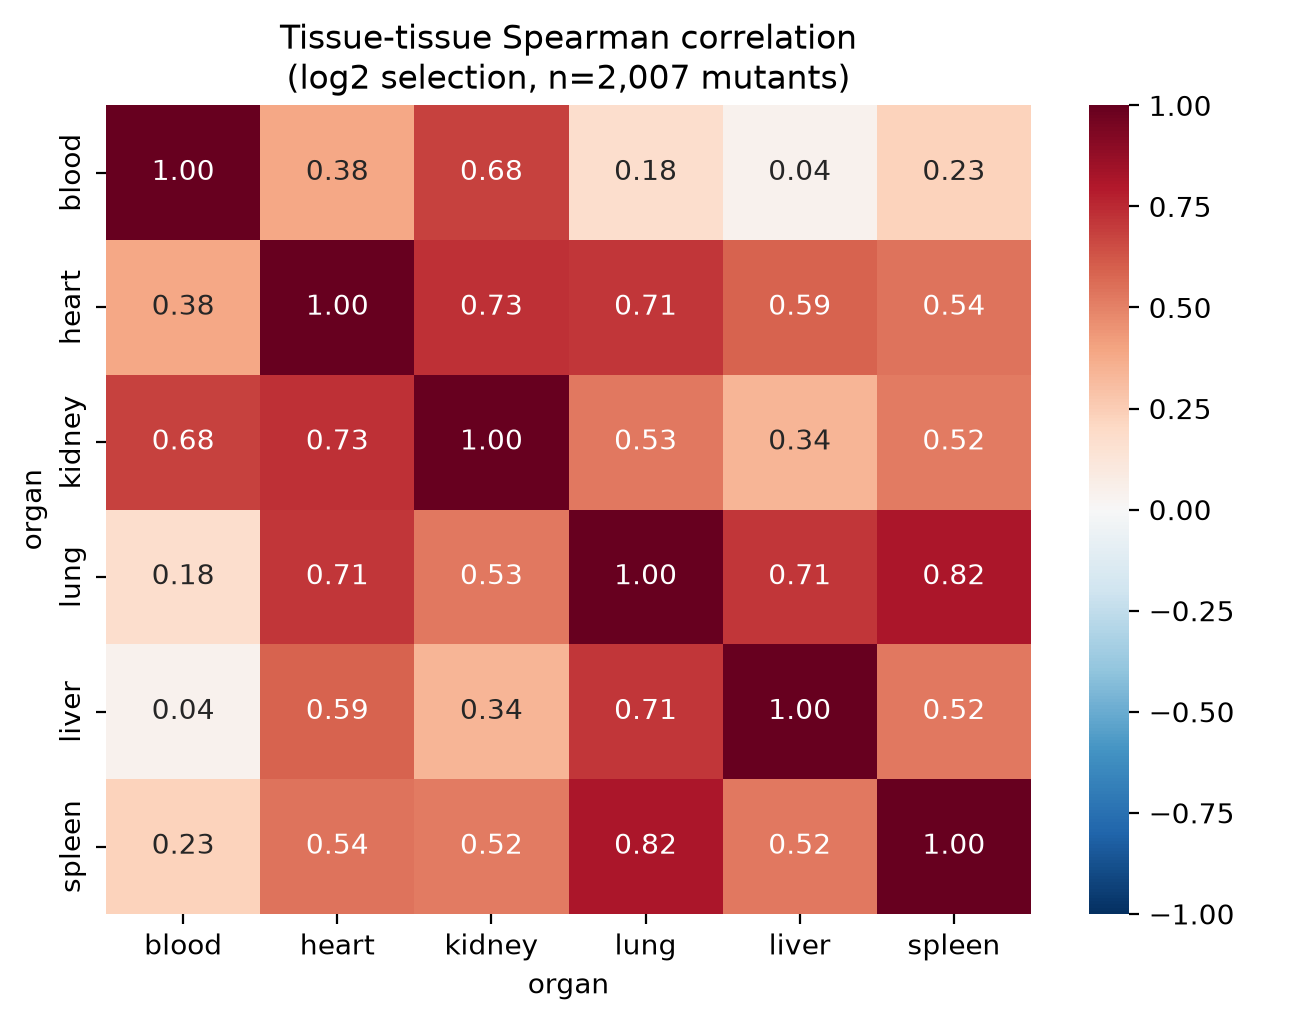
\includegraphics[width=0.62\textwidth]{report_figures/tissue_correlation.png}
\caption{Spearman correlation of log2 selection between tissues, 2,007 mutants.}
\label{fig:tissuecorr}
\end{figure}

\subsection{Symmetry axes}

Positions in contact at the 3-fold axis (n=104) have higher mean absolute selection than the
other positions (n=317): 1.114 vs.\ 0.977 (Mann-Whitney $p=2.9\times10^{-6}$). The fraction of
mutants in the named clusters is also higher: 21.4\% vs.\ 12.7\% ($p=3.1\times10^{-6}$). Ogden
et al.\ state that two of the three clusters lie in surface patches near the 3-fold axis; the
numbers here agree in direction with that statement.

Positions at the 5-fold axis (n=26) have lower mean absolute selection than the other positions
(n=395): 0.652 vs.\ 1.035 ($p=0.014$). The named-cluster fraction is 12.8\% vs.\ 15.0\%
($p=0.125$, not significant). The 5-fold pore has been described as the route for genome
packaging and for externalization of the VP1 N-terminal phospholipase domain
\citep{bleker2005, mietzsch2019}. We have not tested whether this accounts for the lower
selection at these positions.

Only four positions are on the 2-fold axis (0.587 vs.\ 1.015, $p=0.270$; named-cluster fraction
50.0\% vs.\ 14.5\%, $p=0.207$). No conclusion is drawn from that group.

\begin{figure}[H]
\centering
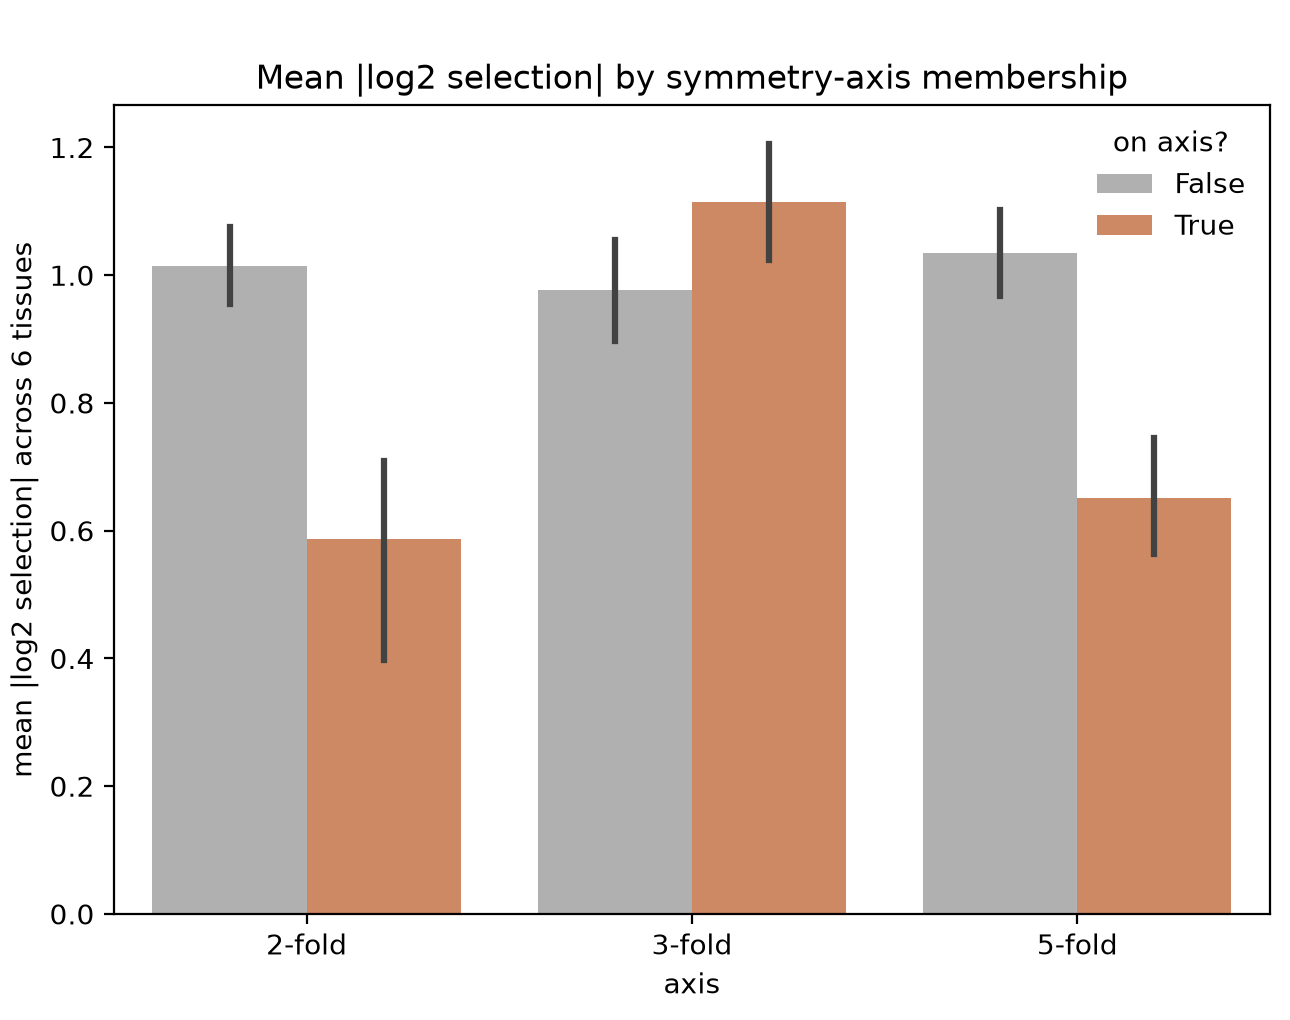
\includegraphics[width=0.55\textwidth]{report_figures/axis_membership.png}
\caption{Mean $|\log_2$ selection$|$ across six tissues, positions on vs.\ off each symmetry
axis. Error bars are the plotting library's default interval. n on axis: 2-fold 4, 3-fold 104,
5-fold 26; 421 positions total.}
\label{fig:axis}
\end{figure}

\subsection{Variable regions, position level}

Positions inside a VR (n=156) have higher mean absolute selection than positions outside (n=265):
1.346 vs.\ 0.814 (Mann-Whitney $p=2.5\times10^{-21}$). Among VR positions, mean absolute
selection differs by region (Kruskal-Wallis $p=1.3\times10^{-16}$; Table~\ref{tab:vrpos}). VR-VI,
VR-V and VR-VIII have the highest means (1.87, 1.72, 1.61). VR-VII (0.646) is lower than the
non-VR mean. VR-II has one position and VR-I and VR-IX have six each, so their means are
imprecise.

Of the 156 VR positions, 42 (26.9\%) are also 3-fold-axis positions, compared with 62 of 265
(23.4\%) non-VR positions. Figure~\ref{fig:track} shows mean absolute selection along the
sequence with the VR intervals and the symmetry-axis positions.

\begin{table}[H]
\centering
\caption{Variable-region boundaries (VP1 numbering) and per-position mean absolute selection.}
\label{tab:vrpos}
\begin{tabular}{lccc}
\toprule
Region & Residues & Positions & Mean $|$selection$|$ \\
\midrule
VR-I & 262--269 & 6 & 1.126 \\
VR-II & 326--331 & 1 & 0.391 \\
VR-IV & 449--469 & 32 & 0.894 \\
VR-V & 487--504 & 34 & 1.720 \\
VR-VI & 525--540 & 26 & 1.869 \\
VR-VII & 544--556 & 20 & 0.646 \\
VR-VIII & 579--594 & 31 & 1.613 \\
VR-IX & 704--711 & 6 & 0.696 \\
Non-VR & all other & 265 & 0.814 \\
\bottomrule
\end{tabular}
\end{table}

\begin{figure}[H]
\centering
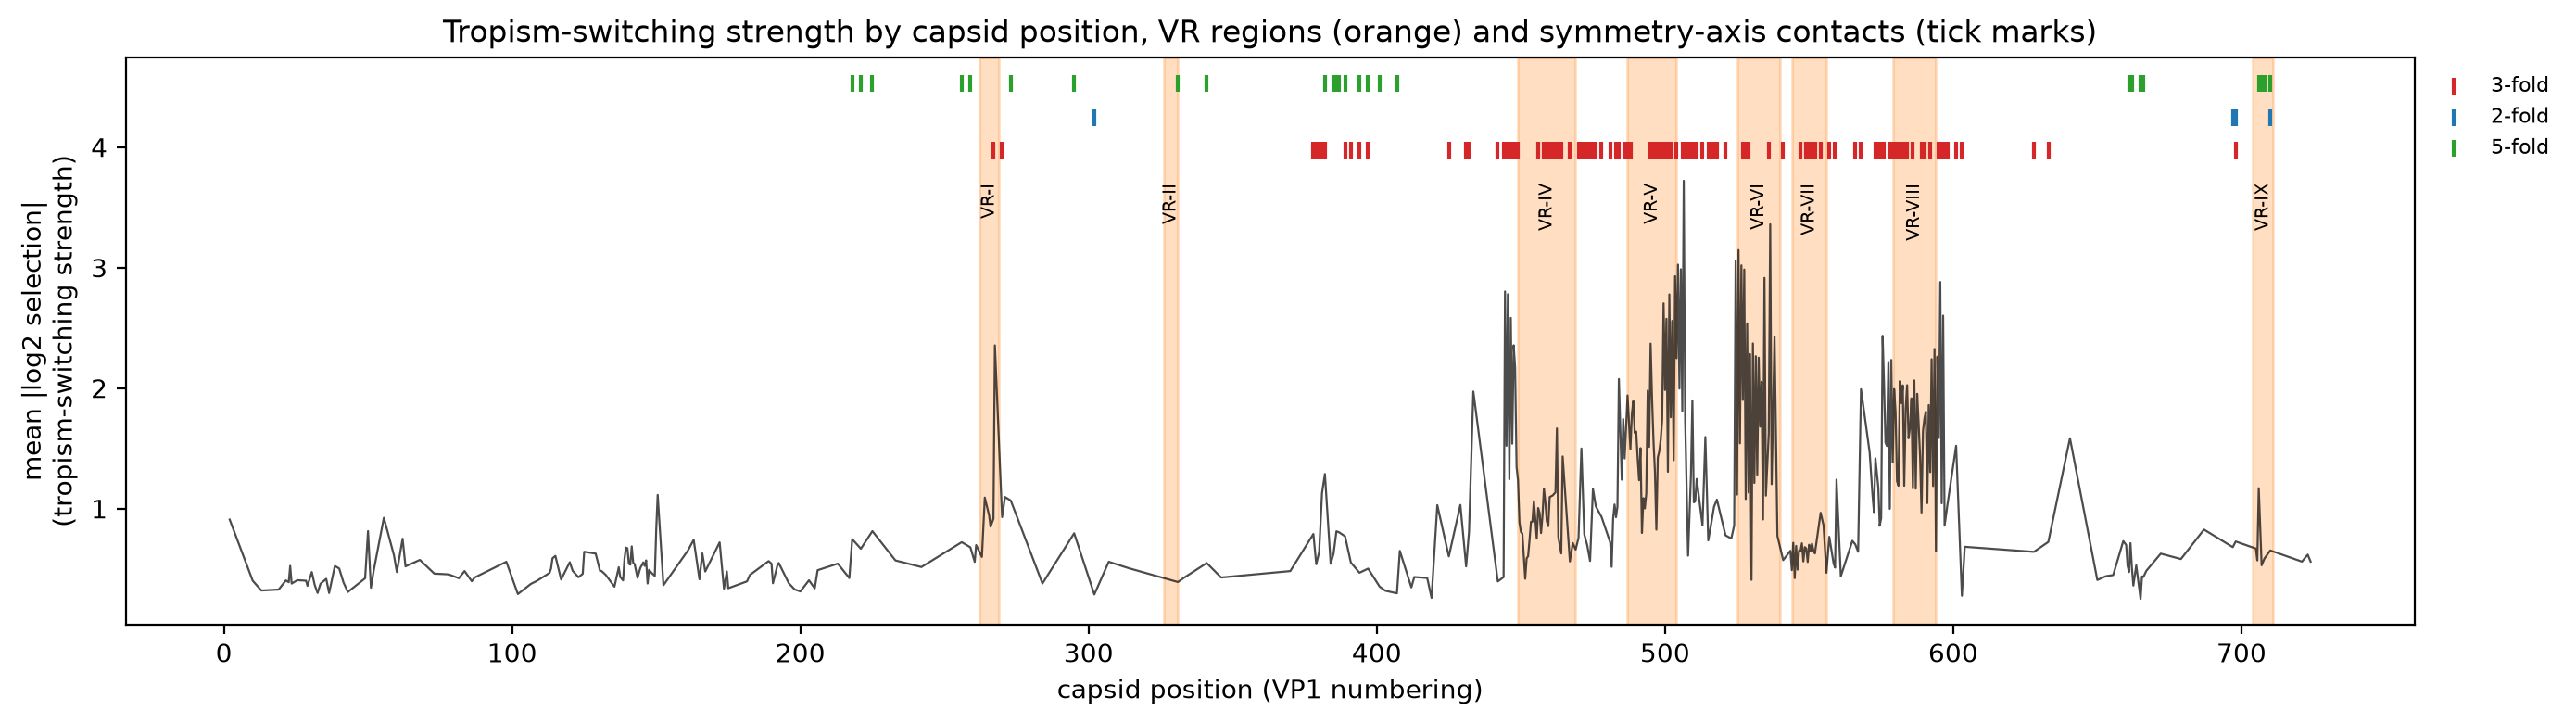
\includegraphics[width=\textwidth]{report_figures/position_hotspot_track.png}
\caption{Mean $|\log_2$ selection$|$ by capsid position. Shaded bands are VRs. Tick marks at the
top show positions in 3-fold (red), 2-fold (blue) and 5-fold (green) axis contacts.}
\label{fig:track}
\end{figure}

\subsection{Variable region effects by tissue}

Table~\ref{tab:vrorgan} and Figure~\ref{fig:vrheat} give the VR coefficients from the organ-level
OLS. Each value is the difference in mean signed log2 selection for mutants inside that VR
relative to mutants outside all VRs, adjusted for the other model terms. 35 of
48 coefficients are stable, compared with 20 of 78 for the property
deltas in the same models.

By region: VR-VII is stable and positive in all six tissues (0.46 to 1.19). VR-IX is stable and
positive in five (not liver). VR-IV is stable and positive in five (not blood). VR-V and VR-VI
are stable and negative in five tissues each (not blood for either). VR-VIII is stable in all six,
positive in blood (1.28), heart (0.30) and kidney (0.62) and negative in liver ($-$0.51), lung
($-$0.74) and spleen ($-$0.70). VR-I is stable in kidney (positive), liver (negative) and spleen
(positive). VR-II (one position) has no stable coefficient.

The position-level and model-level results for VR-VII point in different directions (low mean
absolute selection, Table~\ref{tab:vrpos}, but positive signed coefficients, Table~\ref{tab:vrorgan}).
The two measures differ (absolute vs.\ signed selection; position means vs.\ a mutant-level model
with covariates). We have not reconciled them further.

When the bootstrap is taken over positions instead of mutants (Section~\ref{sec:receptor}), 30 of 48 VR coefficients are stable
(\texttt{vr\_ols\_position\_bootstrap\_no\_receptor\_terms.csv}), compared with 35 of 48 in Table~\ref{tab:vrorgan}.

Insertions and deletions have negative coefficients relative to substitutions in most tissues
(Table~\ref{tab:lib}). The insertion coefficient is stable in heart, kidney, lung, liver and
spleen. The deletion coefficient is stable in heart, lung, liver and spleen. Neither is stable in
blood.

\begin{table}[H]
\centering
\caption{VR indicator coefficients (bootstrap mean, log2 selection units) from the organ-level
OLS. Reference group: mutants outside all VRs. Bold: 95\% bootstrap interval excludes zero.
Source: \texttt{expanded\_organ\_ols\_bootstrap.csv}.}
\label{tab:vrorgan}
\small
\begin{tabular}{lrrrrrr}
\toprule
Region & Blood & Heart & Kidney & Liver & Lung & Spleen \\
\midrule
VR-I & 0.508 & 0.178 & \textbf{0.483} & 0.436 & \textbf{$-$0.412} & \textbf{0.603} \\
VR-II & 0.477 & 0.146 & 0.461 & 0.264 & 0.691 & 0.539 \\
VR-IV & 0.166 & \textbf{0.464} & \textbf{0.468} & \textbf{0.613} & \textbf{0.608} & \textbf{0.191} \\
VR-V & 0.040 & \textbf{$-$0.226} & \textbf{$-$0.214} & \textbf{$-$0.756} & \textbf{$-$0.777} & \textbf{$-$0.530} \\
VR-VI & $-$0.040 & \textbf{$-$0.285} & \textbf{$-$0.434} & \textbf{$-$0.898} & \textbf{$-$0.547} & \textbf{$-$1.184} \\
VR-VII & \textbf{0.590} & \textbf{0.458} & \textbf{0.540} & \textbf{1.194} & \textbf{0.699} & \textbf{0.914} \\
VR-VIII & \textbf{1.283} & \textbf{0.302} & \textbf{0.621} & \textbf{$-$0.745} & \textbf{$-$0.505} & \textbf{$-$0.696} \\
VR-IX & \textbf{0.929} & \textbf{0.621} & \textbf{0.797} & \textbf{0.663} & 0.476 & \textbf{0.692} \\
\bottomrule
\end{tabular}
\end{table}

\begin{figure}[H]
\centering
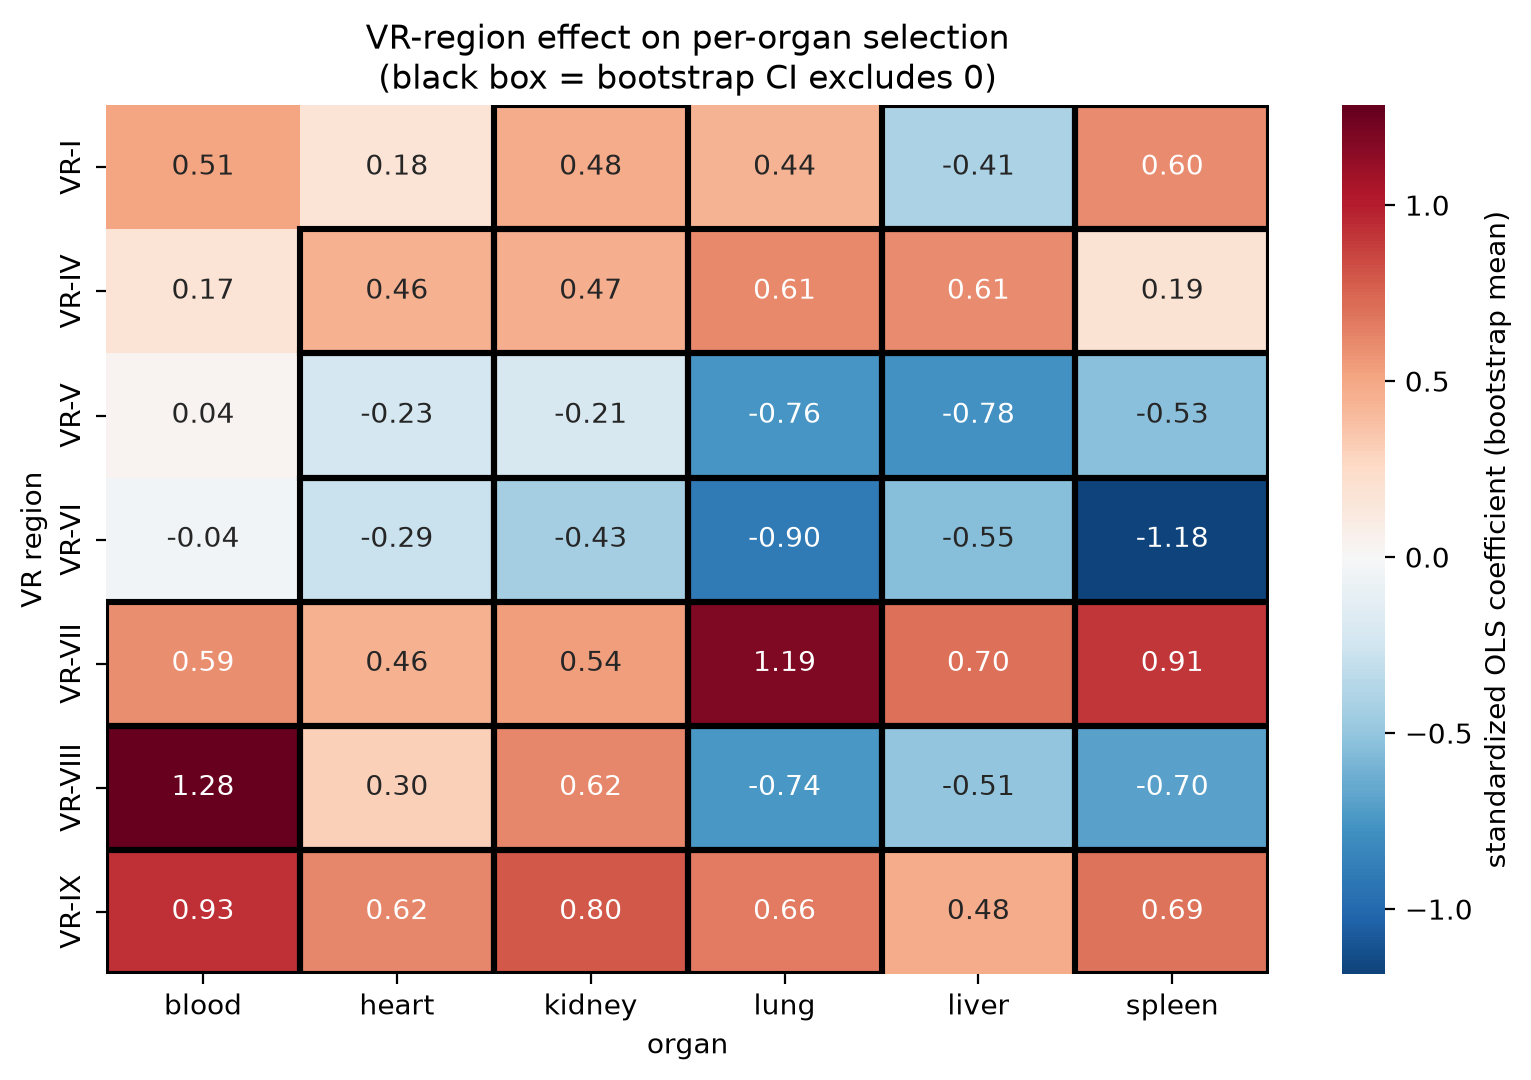
\includegraphics[width=0.85\textwidth]{report_figures/vr_region_organ_heatmap.png}
\caption{VR coefficients from Table~\ref{tab:vrorgan}. Black outlines mark coefficients with a
bootstrap interval that excludes zero. The color bar label in the image says ``standardized''; the
VR and library-type indicators are 0/1 and were not rescaled. Only the property deltas were
z-scored.}
\label{fig:vrheat}
\end{figure}

\begin{table}[H]
\centering
\caption{Library-type coefficients (bootstrap mean) from the same models. Reference: substitution.
Bold: interval excludes zero.}
\label{tab:lib}
\small
\begin{tabular}{lrrrrrr}
\toprule
Type & Blood & Heart & Kidney & Liver & Lung & Spleen \\
\midrule
Insertion & $-$0.048 & \textbf{$-$0.524} & \textbf{$-$0.428} & \textbf{$-$1.096} & \textbf{$-$0.841} & \textbf{$-$0.838} \\
Deletion & 0.236 & \textbf{$-$0.450} & $-$0.205 & \textbf{$-$0.792} & \textbf{$-$0.634} & \textbf{$-$0.555} \\
\bottomrule
\end{tabular}
\end{table}

\subsection{Physicochemical properties and tissue selection}

\textbf{Organ-level OLS coefficients.} Of 78 property-by-tissue coefficients,
20 are stable (Table~\ref{tab:prop}, Figure~\ref{fig:propgrid}). Net charge is
stable and positive in lung and spleen. Helix initiation parameter is stable and negative in lung
and spleen. Apparent partial specific volume is stable and negative in heart and liver. Polarity
is stable and negative in heart and liver and positive in spleen. Coil-frequency and double-bend
frequency are stable and negative in blood.

\begin{table}[H]
\centering
\caption{Stable property-delta coefficients from the organ-level OLS (bootstrap mean and 95\%
percentile interval). Coefficients are per standard deviation of the property delta.}
\label{tab:prop}
\small
\begin{tabular}{llrr}
\toprule
Tissue & Property & Coefficient & 95\% interval \\
\midrule
Blood & Relative frequency of double bend & $-$0.211 & [$-$0.369, $-$0.057] \\
Blood & Relative frequency of coil & $-$0.195 & [$-$0.286, $-$0.099] \\
Blood & AAindex ``A parameter'' scale & 0.119 & [0.040, 0.209] \\
Heart & Apparent partial specific volume & $-$0.195 & [$-$0.303, $-$0.087] \\
Heart & Polarity & $-$0.102 & [$-$0.184, $-$0.025] \\
Heart & 3J(H$\alpha$-NH) coupling constant & 0.068 & [0.009, 0.130] \\
Heart & pK & 0.095 & [0.013, 0.179] \\
Kidney & Relative frequency of coil & $-$0.062 & [$-$0.125, $-$0.001] \\
Lung & Helix initiation parameter & $-$0.168 & [$-$0.303, $-$0.025] \\
Lung & Net charge & 0.173 & [0.070, 0.280] \\
Liver & Apparent partial specific volume & $-$0.296 & [$-$0.488, $-$0.104] \\
Liver & Polarity & $-$0.174 & [$-$0.316, $-$0.034] \\
Liver & Relative frequency of coil & 0.089 & [0.006, 0.170] \\
Liver & Molecular weight & 0.114 & [0.007, 0.222] \\
Spleen & Helix initiation parameter & $-$0.260 & [$-$0.369, $-$0.153] \\
Spleen & pK & $-$0.137 & [$-$0.249, $-$0.029] \\
Spleen & Molecular weight & $-$0.111 & [$-$0.193, $-$0.033] \\
Spleen & 3J(H$\alpha$-NH) coupling constant & $-$0.101 & [$-$0.171, $-$0.037] \\
Spleen & Polarity & 0.112 & [0.013, 0.208] \\
Spleen & Net charge & 0.178 & [0.086, 0.273] \\
\bottomrule
\end{tabular}
\end{table}

\begin{figure}[H]
\centering
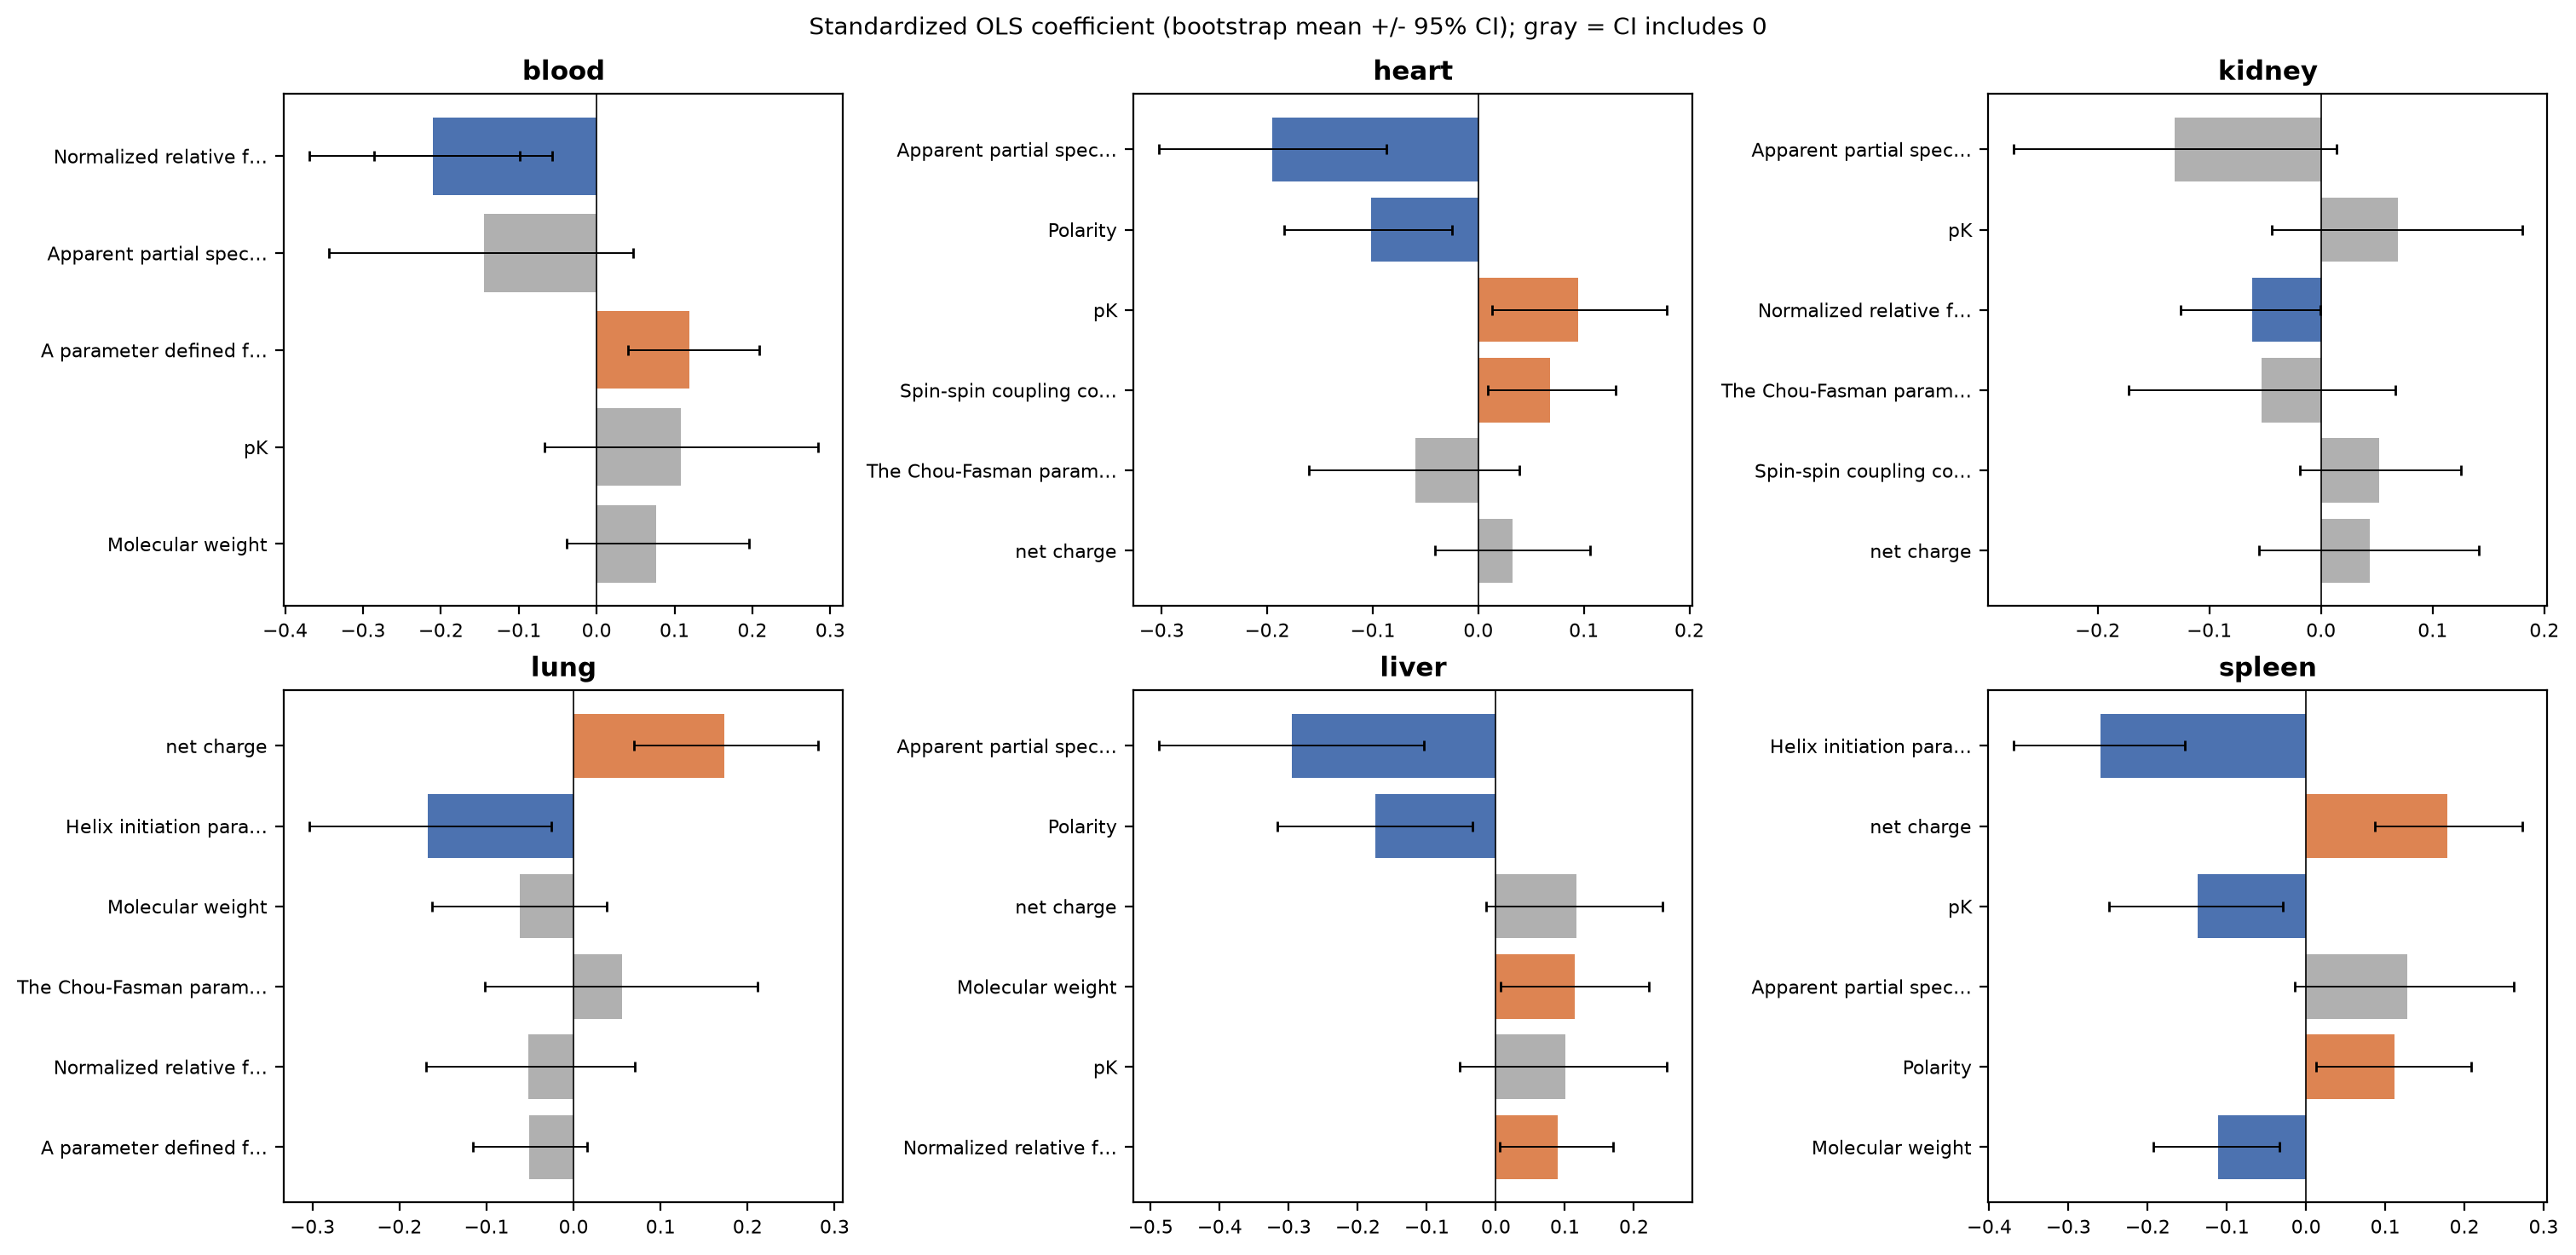
\includegraphics[width=\textwidth]{report_figures/expanded_organ_ols_bootstrap_grid.png}
\caption{Top property coefficients per tissue from the organ-level OLS, with 95\% bootstrap
intervals. Gray bars have intervals that include zero. Only the largest coefficients per tissue
are shown; Table~\ref{tab:prop} lists all stable ones.}
\label{fig:propgrid}
\end{figure}

\textbf{Univariate Spearman correlations.} Table~\ref{tab:sp} gives the Spearman correlation of
each property delta with each tissue's log2 selection across mutants. No significance marking is
shown in this table.

\begin{table}[H]
\centering
\caption{Spearman correlation between property delta and log2 selection, 13-property panel.
Source: \texttt{expanded\_mutation\_organ\_spearman.csv}.}
\label{tab:sp}
\small
\begin{tabular}{lrrrrrr}
\toprule
Property & Blood & Heart & Kidney & Lung & Liver & Spleen \\
\midrule
Alpha-helix index (beta-proteins) & 0.020 & 0.125 & 0.075 & 0.063 & 0.085 & $-$0.001 \\
Helix initiation parameter & $-$0.006 & 0.115 & 0.040 & $-$0.078 & 0.040 & $-$0.208 \\
3J(H$\alpha$-NH) coupling constant & 0.037 & 0.074 & 0.067 & 0.109 & 0.129 & 0.112 \\
Frequency of 4th residue in turn & 0.007 & $-$0.008 & $-$0.024 & 0.001 & 0.026 & 0.031 \\
pK & 0.009 & 0.045 & 0.030 & $-$0.045 & $-$0.050 & $-$0.106 \\
Molecular weight & 0.022 & $-$0.047 & 0.003 & 0.046 & 0.043 & 0.123 \\
Chou-Fasman coil parameter & 0.003 & $-$0.034 & $-$0.030 & $-$0.039 & $-$0.003 & $-$0.041 \\
Relative frequency of coil & 0.027 & 0.003 & $-$0.004 & $-$0.037 & 0.001 & $-$0.063 \\
Apparent partial specific volume & $-$0.011 & $-$0.069 & $-$0.018 & 0.004 & $-$0.085 & 0.040 \\
Polarity & 0.003 & $-$0.079 & $-$0.035 & $-$0.073 & $-$0.024 & $-$0.013 \\
Relative frequency of double bend & $-$0.085 & $-$0.076 & $-$0.075 & $-$0.050 & 0.001 & 0.026 \\
AAindex ``A parameter'' scale & 0.060 & $-$0.003 & 0.021 & 0.014 & 0.018 & 0.034 \\
Net charge & $-$0.010 & $-$0.139 & $-$0.060 & 0.076 & $-$0.062 & 0.205 \\
\bottomrule
\end{tabular}
\end{table}

\textbf{Fit of the 4-property and 13-property models.} Table~\ref{tab:r2} and
Figure~\ref{fig:r2} compare the in-sample $R^2$ of OLS models using only the property deltas
(no VR or library-type terms). The 13-property model has a higher $R^2$ in all six tissues, by
0.003 (lung) to 0.033 (blood). The 4-property and 13-property sets are not nested (the 4-property
set includes hydrophobicity and residue volume, which are not in the 13), and the $R^2$ values
are in-sample, not cross-validated.

\begin{table}[H]
\centering
\caption{In-sample $R^2$, property-only OLS.}
\label{tab:r2}
\begin{tabular}{lccc}
\toprule
Tissue & 4 properties & 13 properties & Difference \\
\midrule
Blood & 0.138 & 0.172 & $+$0.033 \\
Heart & 0.220 & 0.228 & $+$0.008 \\
Kidney & 0.161 & 0.168 & $+$0.007 \\
Lung & 0.347 & 0.350 & $+$0.003 \\
Liver & 0.237 & 0.241 & $+$0.004 \\
Spleen & 0.346 & 0.362 & $+$0.016 \\
\bottomrule
\end{tabular}
\end{table}

\begin{figure}[H]
\centering
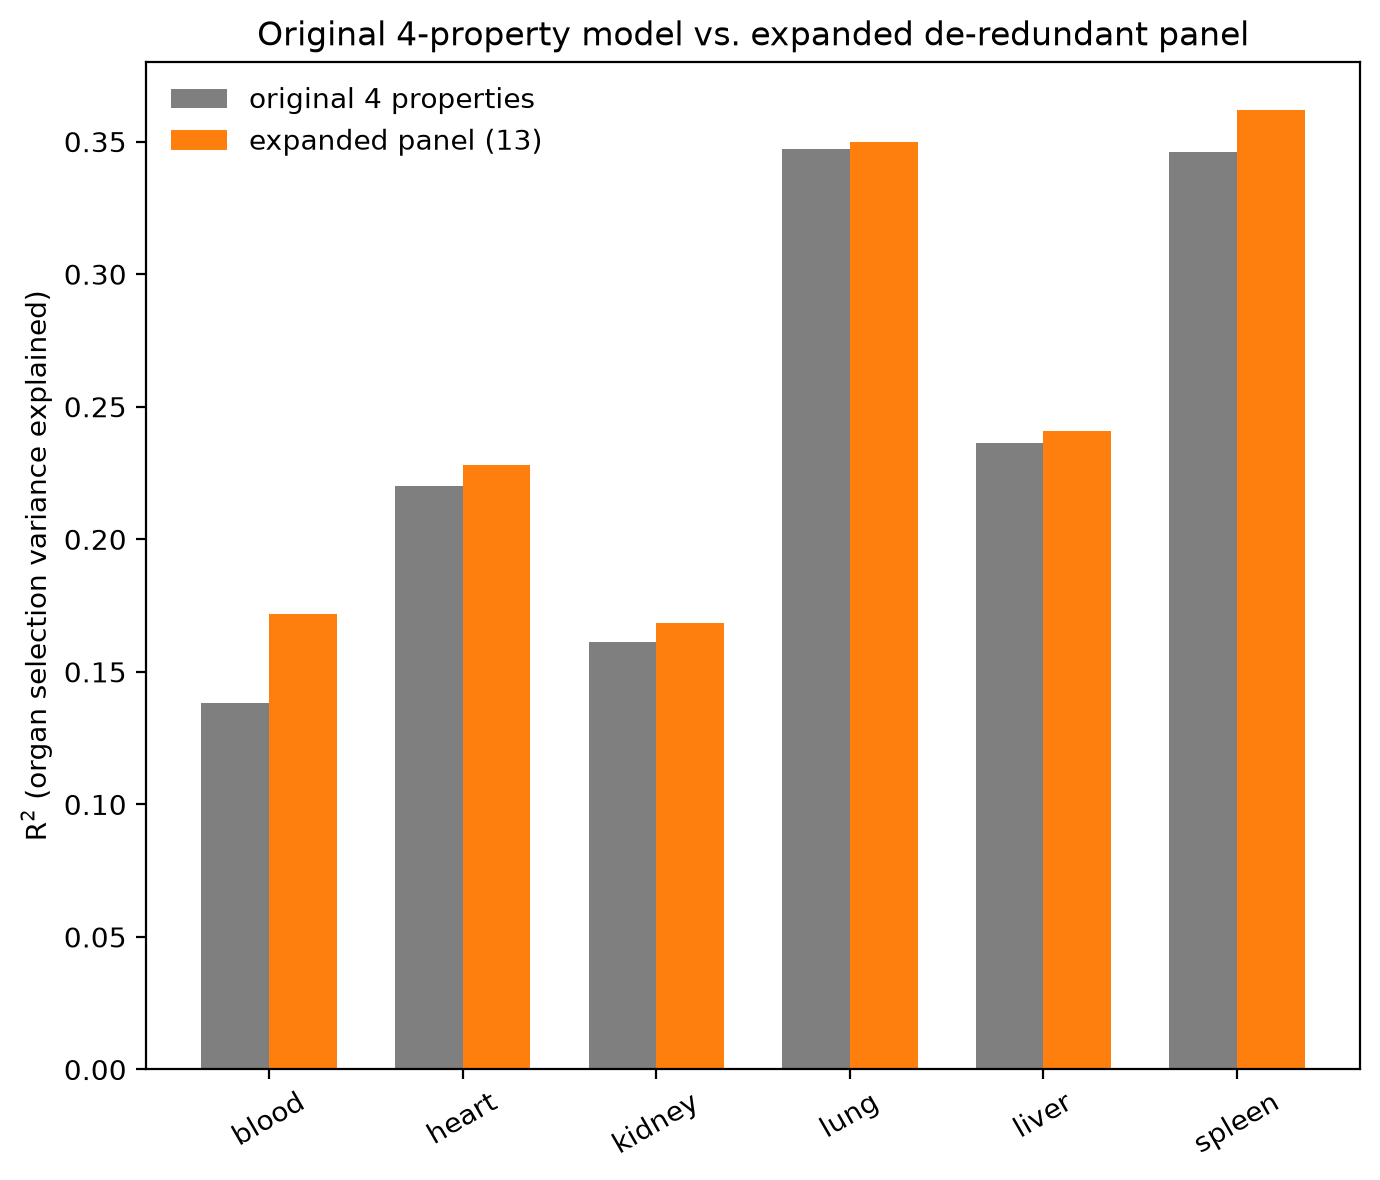
\includegraphics[width=0.6\textwidth]{report_figures/expanded_r2_comparison.png}
\caption{In-sample $R^2$ per tissue for the 4-property and 13-property models.}
\label{fig:r2}
\end{figure}

\subsection{PCovC feature weights by cluster}

Table~\ref{tab:pxz} lists the $p_{xz}$ weights whose bootstrap intervals exclude zero (7, 7, 5 and
5 of 25 features for the other class and clusters 1, 2 and 3, respectively). Figure~\ref{fig:pxz}
shows the top weights for clusters 1 to 3.

For cluster 1, net charge (negative) and apparent partial specific volume (negative) are stable,
as are VR-VIII (positive) and VR-VII (negative). For clusters 2 and 3, the Chou-Fasman coil
parameter and polarity are both stable with opposite signs (cluster 2: 0.061 and 0.050; cluster
3: $-$0.065 and $-$0.057). Apparent partial specific volume is stable and positive for cluster 3
(0.073) and stable and negative for cluster 1 ($-$0.095). The stable weights are small in absolute
size (largest magnitude 0.164), and many intervals have a bound close to zero.

\begin{table}[H]
\centering
\caption{Stable $p_{xz}$ weights (bootstrap mean and 95\% percentile interval).}
\label{tab:pxz}
\small
\begin{tabular}{llrr}
\toprule
Class & Feature & Weight & 95\% interval \\
\midrule
Other & VR-VIII indicator & $-$0.068 & [$-$0.120, $-$0.006] \\
 & VR-VI indicator & $-$0.025 & [$-$0.048, $-$0.002] \\
 & VR-V indicator & $-$0.024 & [$-$0.050, $-$0.001] \\
 & VR-I indicator & 0.009 & [0.000, 0.018] \\
 & VR-VII indicator & 0.053 & [0.003, 0.100] \\
 & Apparent partial specific volume & 0.074 & [0.009, 0.128] \\
 & Net charge & 0.135 & [0.001, 0.215] \\
\midrule
Cluster 1 & Net charge & $-$0.164 & [$-$0.280, $-$0.004] \\
 & Apparent partial specific volume & $-$0.095 & [$-$0.180, $-$0.007] \\
 & VR-VII indicator & $-$0.065 & [$-$0.126, $-$0.005] \\
 & VR-I indicator & $-$0.010 & [$-$0.021, $-$0.000] \\
 & VR-V indicator & 0.029 & [0.002, 0.064] \\
 & VR-VI indicator & 0.030 & [0.003, 0.062] \\
 & VR-VIII indicator & 0.083 & [0.008, 0.156] \\
\midrule
Cluster 2 & Substitution indicator & $-$0.017 & [$-$0.041, $-$0.000] \\
 & Insertion indicator & 0.011 & [0.001, 0.028] \\
 & Frequency of 4th residue in turn & 0.026 & [0.001, 0.051] \\
 & Polarity & 0.050 & [0.007, 0.096] \\
 & Chou-Fasman coil parameter & 0.061 & [0.003, 0.124] \\
\midrule
Cluster 3 & Chou-Fasman coil parameter & $-$0.065 & [$-$0.130, $-$0.002] \\
 & Polarity & $-$0.057 & [$-$0.113, $-$0.003] \\
 & Insertion indicator & $-$0.013 & [$-$0.029, $-$0.001] \\
 & Substitution indicator & 0.021 & [0.002, 0.046] \\
 & Apparent partial specific volume & 0.073 & [0.008, 0.144] \\
\bottomrule
\end{tabular}
\end{table}

\begin{figure}[H]
\centering
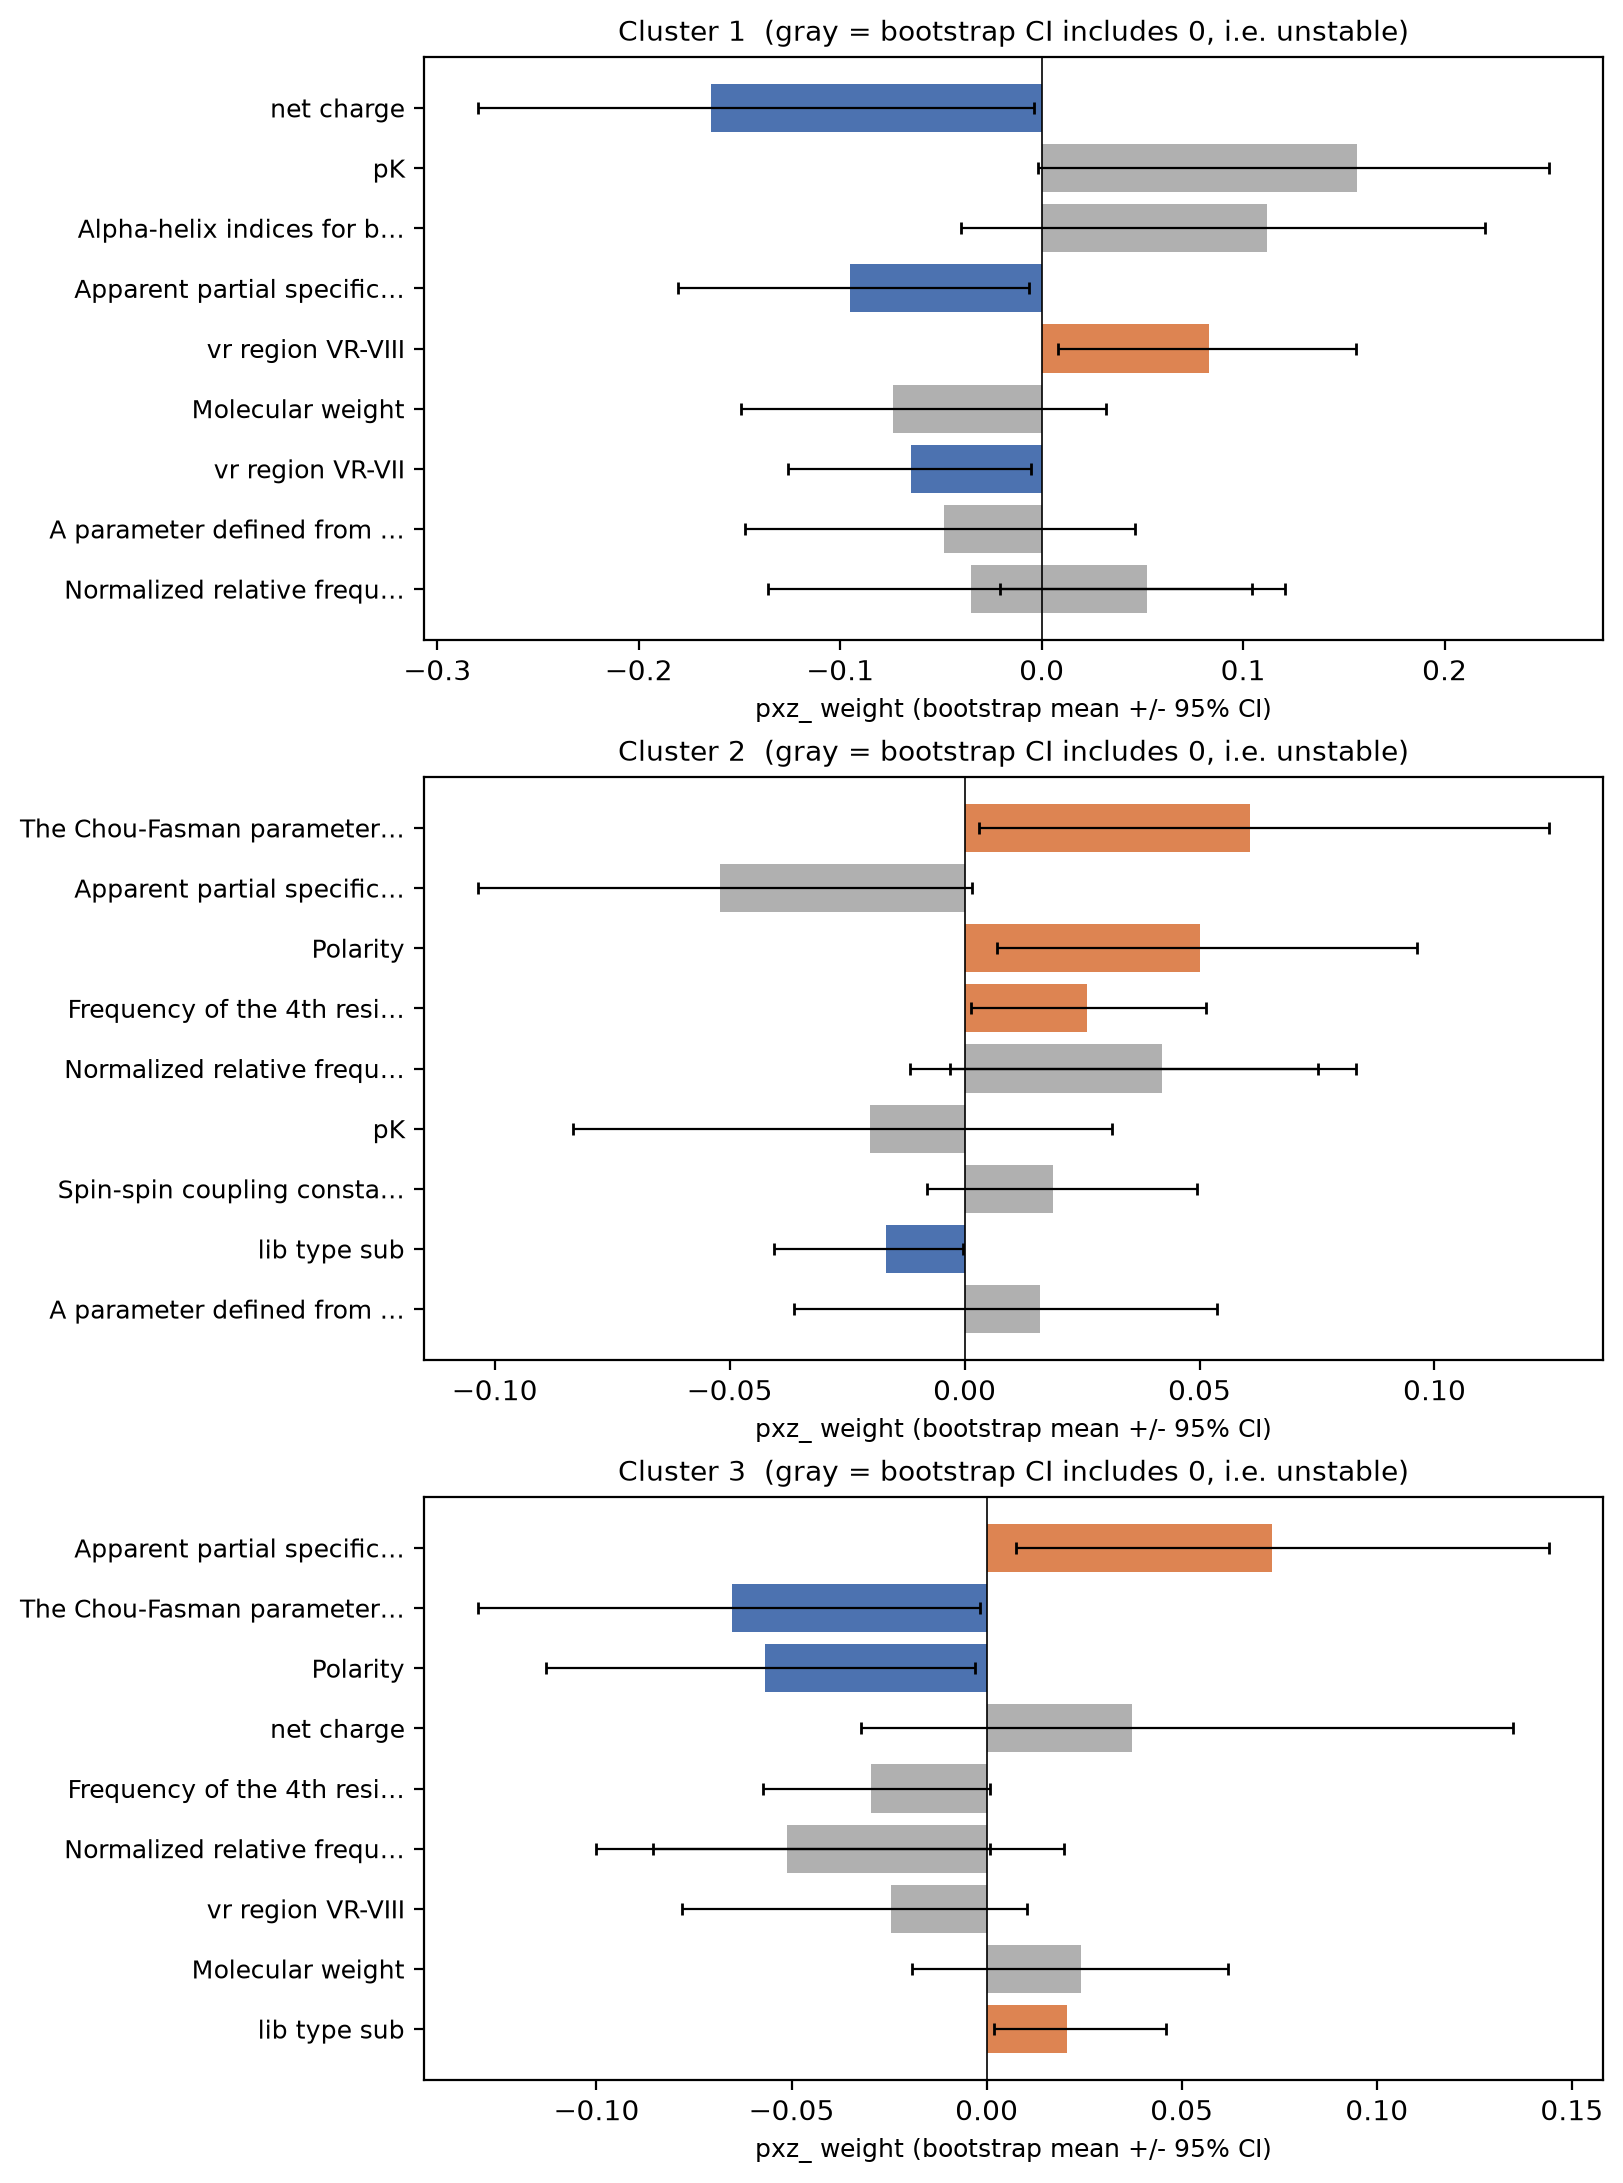
\includegraphics[width=0.62\textwidth]{report_figures/expanded_pxz_bootstrap.png}
\caption{Top $p_{xz}$ weights for clusters 1 to 3 with 95\% bootstrap intervals. Gray bars have
intervals that include zero.}
\label{fig:pxz}
\end{figure}

\subsection{Network centrality and solvent accessibility}

Betweenness centrality is negatively correlated with mean absolute selection for substitutions
(n=1,024, Spearman $\rho=-0.135$, 95\% interval [$-$0.194, $-$0.068], $p=1.4\times10^{-5}$) and
positively correlated for insertions (n=761, $\rho=+0.214$ [0.144, 0.286], $p=2.3\times10^{-9}$).
For deletions (n=37), $\rho=+0.297$ [$-$0.058, 0.553], $p=0.075$. Per-tissue correlations are in
Table~\ref{tab:cent}. A pooled model with a centrality-by-library-type interaction gives a
centrality slope of $-$0.044 [$-$0.079, $-$0.009] for substitutions, with additional slopes of
+0.265 [0.182, 0.344] for insertions and +0.287 [0.067, 0.497] for deletions
(Figure~\ref{fig:centlib}). We do not have an explanation for the difference in sign between
substitutions and insertions.

RSA and centrality are negatively correlated across the 519 positions that have both
($\rho=-0.295$, $p=6.8\times10^{-12}$; Figure~\ref{fig:rsa}). RSA is negatively correlated with
mean absolute selection for substitutions ($\rho=-0.254$ [$-$0.310, $-$0.199]) and insertions
($\rho=-0.388$ [$-$0.444, $-$0.327]). For deletions the estimate is similar
($\rho=-0.266$) but the interval includes zero ([$-$0.569, 0.092], $p=0.112$, n=37).

\begin{table}[H]
\centering
\caption{Spearman correlation of betweenness centrality with mean absolute selection and with
each tissue's log2 selection, by library type (n in parentheses). Bold: 95\% bootstrap interval
excludes zero.}
\label{tab:cent}
\small
\begin{tabular}{lrrrrrrr}
\toprule
Type & Mean $|$sel$|$ & Blood & Heart & Kidney & Lung & Liver & Spleen \\
\midrule
Substitution (1024) & \textbf{$-$0.135} & $-$0.004 & $-$0.018 & \textbf{0.128} & \textbf{$-$0.157} & \textbf{$-$0.191} & \textbf{$-$0.217} \\
Insertion (761) & \textbf{0.214} & \textbf{0.214} & \textbf{0.260} & \textbf{0.220} & \textbf{0.135} & 0.028 & \textbf{0.223} \\
Deletion (37) & 0.297 & 0.182 & 0.242 & 0.225 & 0.250 & 0.302 & 0.142 \\
\bottomrule
\end{tabular}
\end{table}

\begin{figure}[H]
\centering
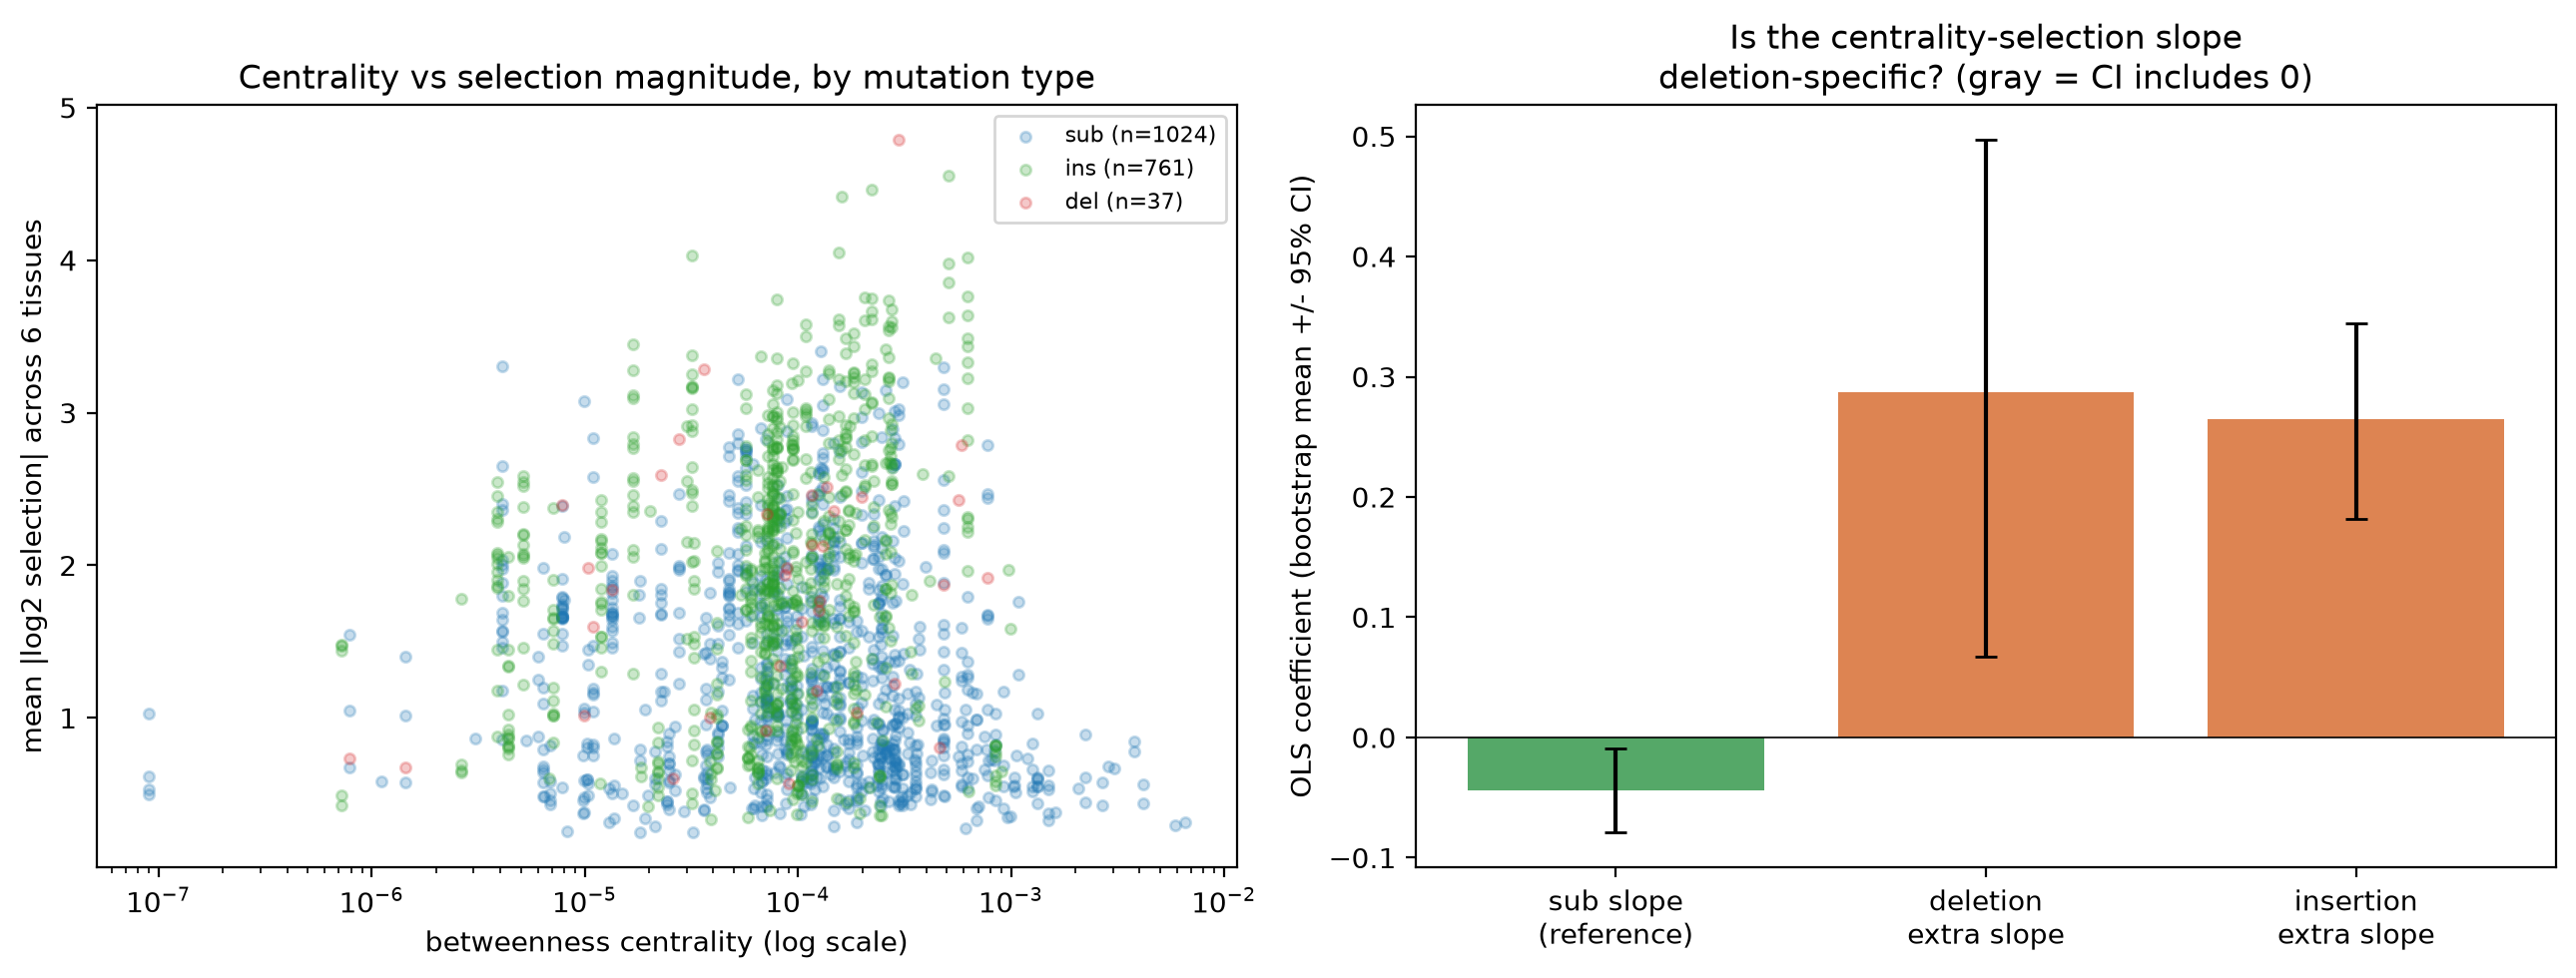
\includegraphics[width=\textwidth]{report_figures/centrality_lib_type_interaction.png}
\caption{Left: centrality vs.\ mean absolute selection by library type. Right: interaction-model
coefficients; the bars are the extra slope for deletions and insertions relative to the
substitution slope, with 95\% bootstrap intervals.}
\label{fig:centlib}
\end{figure}

\begin{figure}[H]
\centering
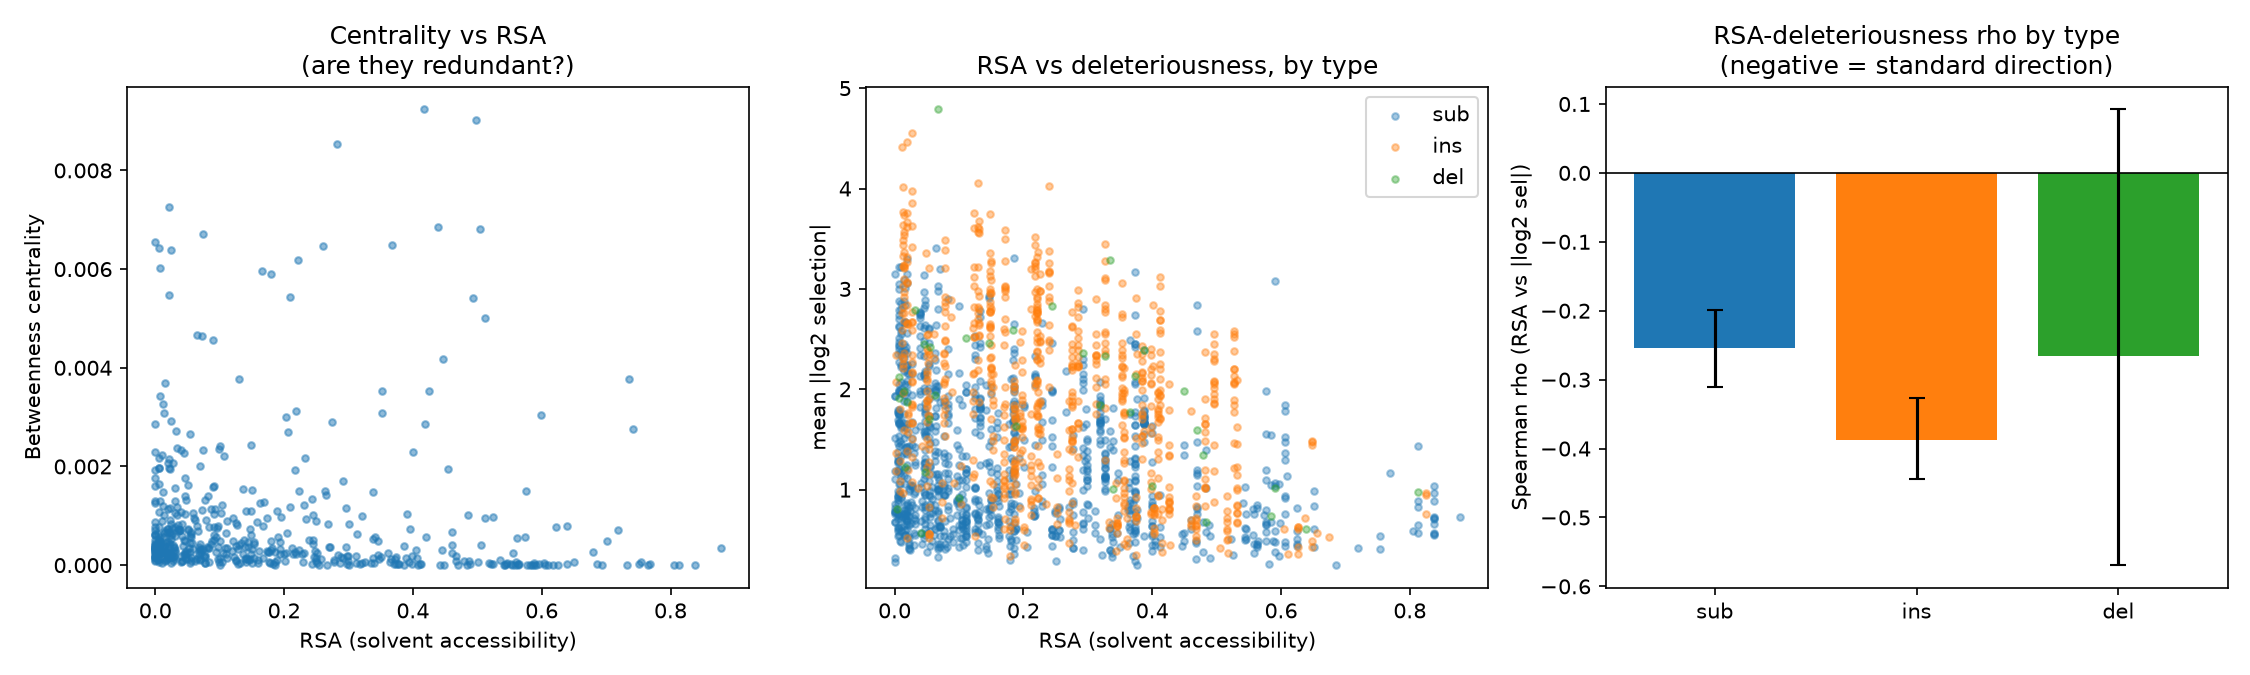
\includegraphics[width=\textwidth]{report_figures/centrality_vs_burial_diagnostic.png}
\caption{Left: centrality vs.\ RSA per position. Middle: RSA vs.\ mean absolute selection by
library type. Right: Spearman correlation of RSA with mean absolute selection by library type,
with 95\% bootstrap intervals.}
\label{fig:rsa}
\end{figure}

\begin{figure}[H]
\centering
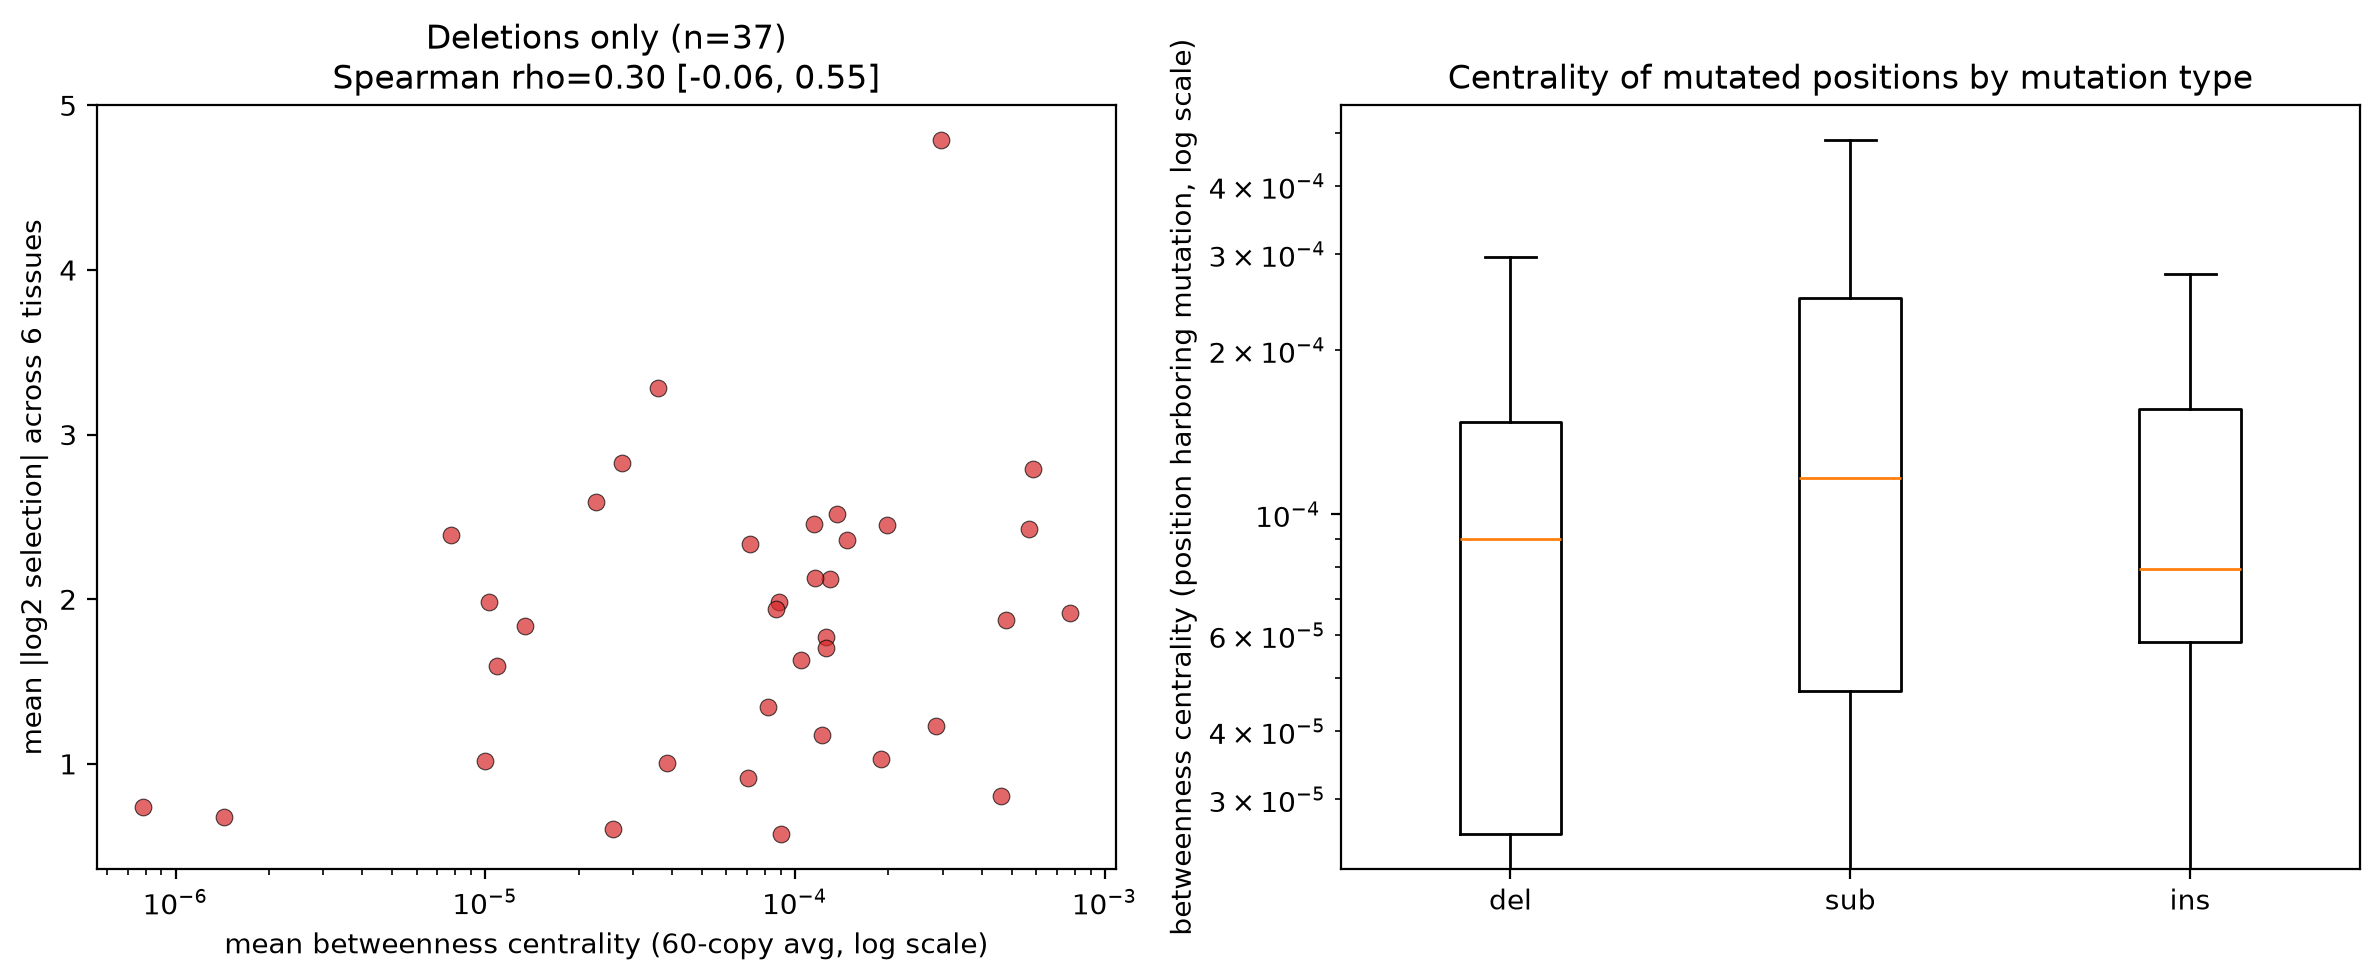
\includegraphics[width=\textwidth]{report_figures/residue_network_centrality.png}
\caption{Left: deletion mutants only, centrality vs.\ mean absolute selection (n=37). Right:
centrality of positions carrying each mutation type.}
\label{fig:delcent}
\end{figure}

\subsection{Receptor-associated residues}
\label{sec:receptor}

The VR results above show that mutations in some regions shift selection differently across
tissues. This section asks whether specific residues that the literature assigns to receptor
binding account for part of that, beyond the region they sit in.

\textbf{Residue sets.} Both sets are in VP1 numbering.
\begin{itemize}
\item \emph{HSPG (heparan sulfate proteoglycan):} R484, R487, K532, R585, R588
  \citep{opie2003, kern2003}. In those studies, mutation of R585 or R588 eliminated binding to
  heparin-agarose, and R484, R487 and K532 mutants kept partial binding. K527 is not included:
  Opie et al.\ report that it does not appear to be involved in heparin binding. The text of the
  AAV2-AAVR structure paper names ``Arg585 and Arg587'' in this context; we use R588, following
  Opie et al.\ and Kern et al.
\item \emph{AAVR (KIAA0319L):} the 19 AAV2 residues with a non-hydrogen atom within 4.5~\AA{} of
  AAVR in the AAV2-AAVR PKD2 complex (Table~2 of \citealt{meyer2019}). That paper describes VR-I
  and VR-III as the core of the footprint. Table~\ref{tab:rvmap} places each residue in the VR
  scheme used here. VR-III is not one of the regions in our model.
\end{itemize}

\begin{table}[H]
\centering
\caption{Receptor-associated residues by variable region. $^\dagger$No mutants for this residue
in the data. Positions H271 and R471 lie just outside VR-I and VR-IV; R484 lies just outside VR-V.}
\label{tab:rvmap}
\small
\begin{tabular}{lll}
\toprule
Region & HSPG residues & AAVR contact residues \\
\midrule
VR-I & none & Q263, S264, G265$^\dagger$, A266, S267, N268$^\dagger$ \\
VR-II & none & none \\
VR-III (not in model) & none & N382, G383$^\dagger$, S384, Q385 \\
VR-IV & none & none \\
VR-V & R487 & W502, T503 \\
VR-VI & K532 & D528, D529 \\
VR-VII & none & none \\
VR-VIII & R585, R588 & Q589 \\
VR-IX & none & K706, V708 \\
Outside VRs & R484 & H271, R471 \\
\bottomrule
\end{tabular}
\end{table}

\textbf{Tests.} Two comparisons were made, both against the region the residue sits in so that
the result does not just restate the VR enrichment. (1) Position level: the mean over positions
of $|$selection$|$ and of signed selection per tissue for the receptor residues, compared with
the same number of residues drawn at random from the same VR strata (20,000 draws; residues
outside all VRs form their own stratum). (2) Mutant level: the organ-level OLS from above with
two added 0/1 indicators (HSPG residue, AAVR residue). Because mutants at one position are not
independent, the bootstrap here resamples positions, with all mutants at a position kept
together (1,000 draws). Mutants of every type at these integer positions are used; insertions
carry half-integer position labels and are not counted. The HSPG set has 5 positions and 87
mutants. The AAVR set has 16 positions with data and 69 mutants (9 of the 16 have three or fewer
mutants).

For reading the numbers: the mean log2 selection of substitution mutants outside all VRs is
negative in every tissue (blood $-$0.90, heart $-$0.70, kidney $-$0.79, lung $-$1.30, liver
$-$1.03, spleen $-$0.85; \texttt{non\_vr\_substitution\_baseline.csv}), so a value near zero is
better than a typical mutant.

\textbf{HSPG residues.} Figure~\ref{fig:rresheat} shows the per-residue means. R585 and R588
(20 mutants each) have the highest blood values of any residue in either set (2.7 for both),
positive values in heart (0.5, 0.6) and kidney (0.5, 0.5), and negative values in lung, liver and
spleen ($-$1.6 to $-$2.6). R487 and K532 are also positive in blood (1.5, 1.1). R484 (10 mutants,
outside all VRs) is 0.8 in blood and has the lowest lung value ($-$3.5); its spleen value is $-$3.1.

Against residues drawn from the same VRs (Table~\ref{tab:rperm}), the HSPG residues have higher
mean absolute selection (1.73 vs.\ 1.27, $p=0.011$), higher blood selection (1.74 vs.\ $-$0.23,
$p<0.001$), higher heart selection ($-$0.04 vs.\ $-$0.69, $p=0.005$) and lower spleen selection
($-$2.88 vs.\ $-$1.41, $p<0.001$). Lung is lower ($p=0.059$). Kidney and liver do not differ from
region-matched residues. In the OLS (Table~\ref{tab:rols}, Figure~\ref{fig:rcoef}), the HSPG
indicator is stable in blood (+2.62), heart (+0.77) and spleen ($-$0.80). Kidney is +0.57 with an
interval that includes zero ([$-$0.24, 1.19]); lung and liver are near zero with wide intervals.

Liver: R585 and R588 are negative in liver ($-$1.8, $-$1.9), but so are the other residues in
these regions, and the HSPG indicator for liver is $-$0.08 [$-$1.01, 0.76]. In this data the HSPG
residues are not distinguishable from their region-mates in liver.

\begin{figure}[H]
\centering
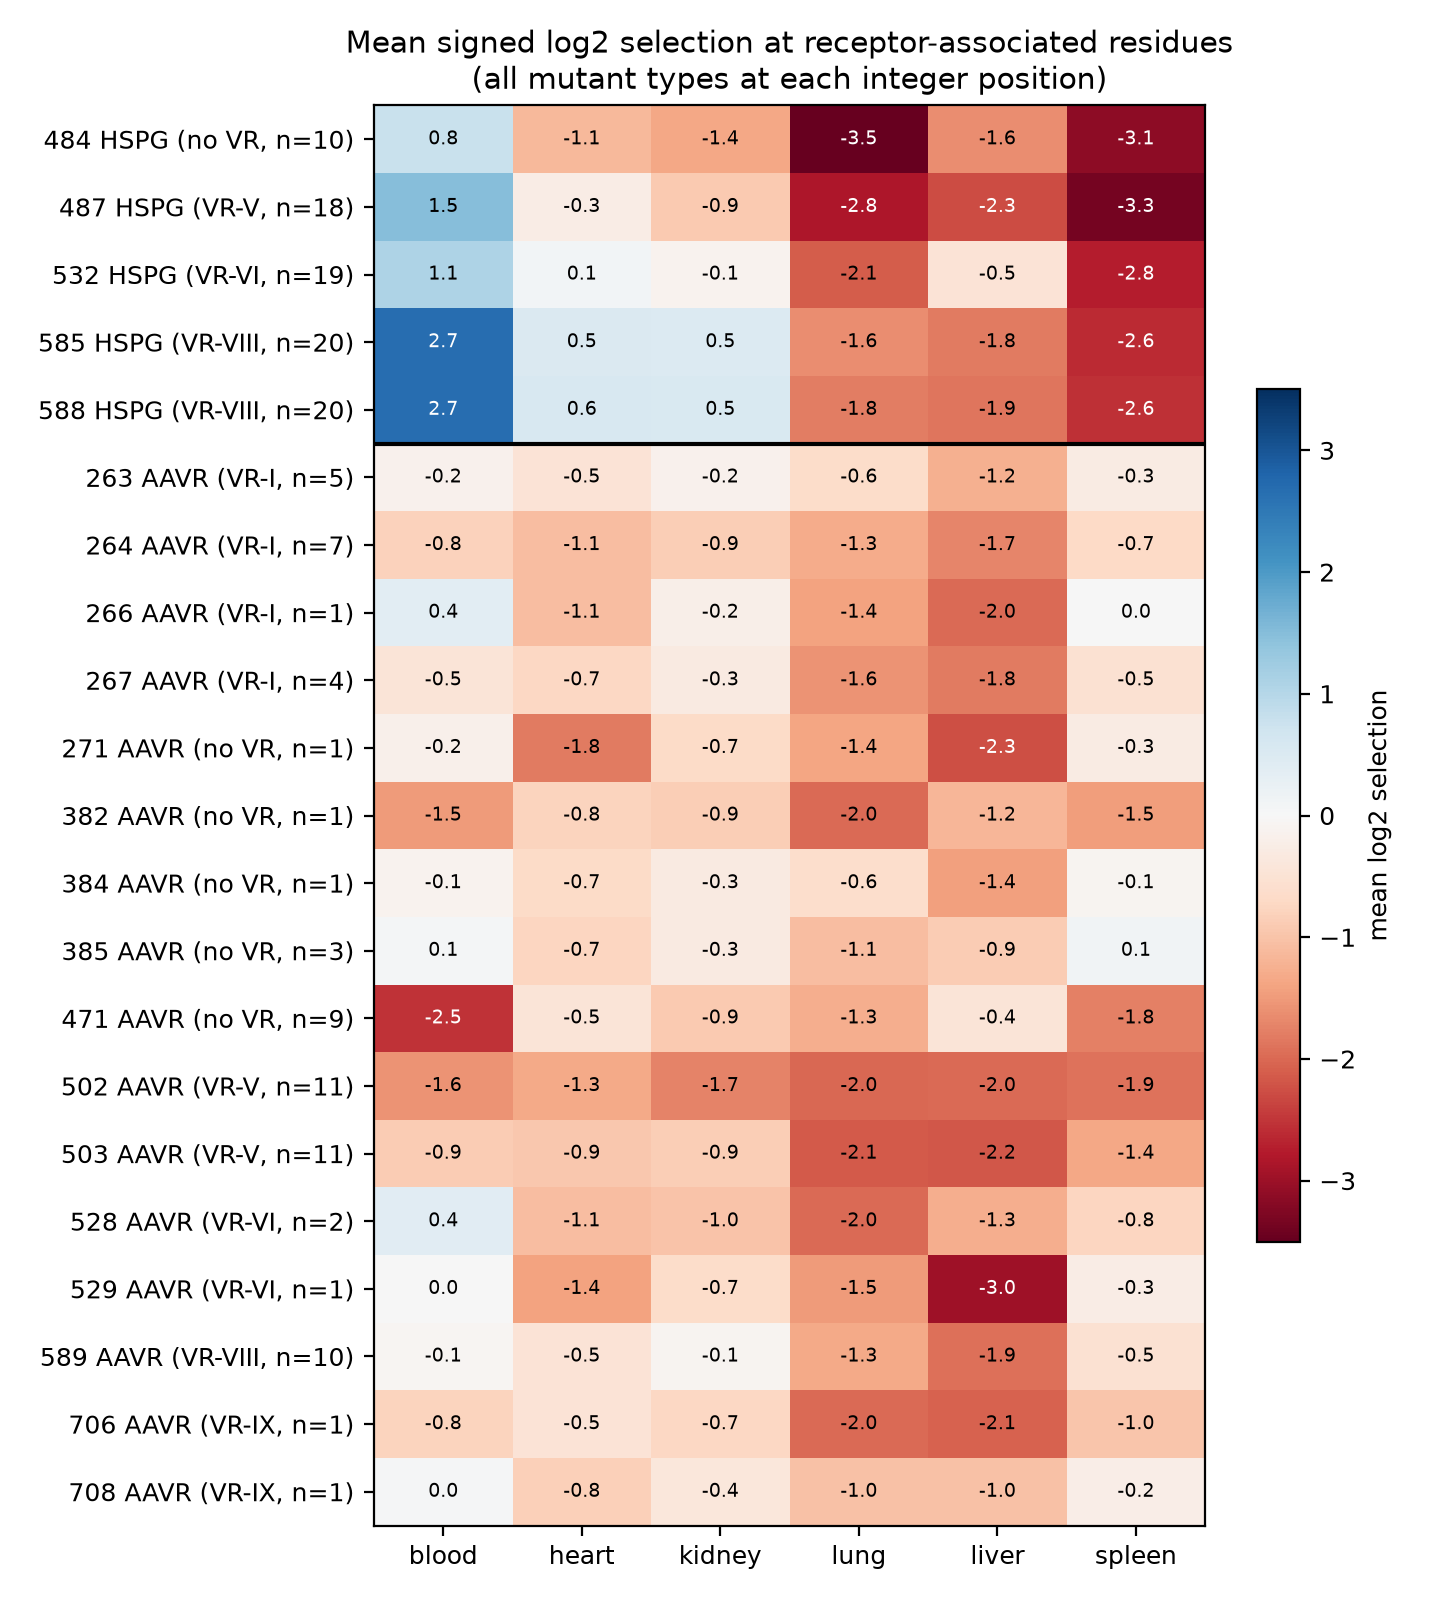
\includegraphics[width=0.82\textwidth]{report_figures/receptor_residue_heatmap.png}
\caption{Mean signed log2 selection per tissue at each receptor-associated residue. Rows above the
black line are HSPG residues; rows below are AAVR contact residues. Labels give the VR and the
number of mutants.}
\label{fig:rresheat}
\end{figure}

\begin{table}[H]
\centering
\caption{Position-level comparison of receptor residues with residues drawn at random from the
same VR strata (20,000 draws). ``VR-matched'' is the mean of the draws. $p$ is two-sided from the
draws.}
\label{tab:rperm}
\small
\begin{tabular}{llrrrr}
\toprule
Set & Measure & Observed & VR-matched & Difference & $p$ \\
\midrule
HSPG (5 positions) & Mean $|$selection$|$ & 1.73 & 1.27 & 0.46 & 0.011 \\
 & Blood & 1.74 & $-$0.23 & 1.97 & $<$0.001 \\
 & Heart & $-$0.04 & $-$0.68 & 0.64 & 0.005 \\
 & Kidney & $-$0.27 & $-$0.66 & 0.39 & 0.118 \\
 & Lung & $-$2.38 & $-$1.78 & $-$0.60 & 0.059 \\
 & Liver & $-$1.62 & $-$1.41 & $-$0.21 & 0.563 \\
 & Spleen & $-$2.88 & $-$1.41 & $-$1.47 & $<$0.001 \\
\midrule
AAVR (16 positions) & Mean $|$selection$|$ & 1.04 & 0.98 & 0.05 & 0.513 \\
 & Blood & $-$0.51 & $-$0.37 & $-$0.14 & 0.478 \\
 & Heart & $-$0.90 & $-$0.70 & $-$0.19 & 0.057 \\
 & Kidney & $-$0.63 & $-$0.58 & $-$0.05 & 0.665 \\
 & Lung & $-$1.45 & $-$1.34 & $-$0.11 & 0.435 \\
 & Liver & $-$1.65 & $-$1.32 & $-$0.33 & 0.057 \\
 & Spleen & $-$0.69 & $-$0.77 & 0.09 & 0.501 \\
\bottomrule
\end{tabular}
\end{table}

\begin{table}[H]
\centering
\caption{Receptor-residue indicator coefficients in the organ-level OLS (bootstrap mean and 95\%
interval, bootstrap over positions). The model also contains the 13 property deltas, the VR
indicators and the library-type indicators. Bold: interval excludes zero.}
\label{tab:rols}
\small
\begin{tabular}{lll}
\toprule
Tissue & HSPG residues & AAVR residues \\
\midrule
Blood & \textbf{2.62 [2.06, 3.14]} & $-$0.07 [$-$0.63, 0.64] \\
Heart & \textbf{0.77 [0.03, 1.21]} & $-$0.08 [$-$0.38, 0.15] \\
Kidney & 0.57 [$-$0.24, 1.19] & $-$0.01 [$-$0.44, 0.35] \\
Lung & 0.06 [$-$1.09, 0.91] & 0.20 [$-$0.21, 0.63] \\
Liver & $-$0.08 [$-$1.01, 0.76] & $-$0.11 [$-$0.54, 0.33] \\
Spleen & \textbf{$-$0.80 [$-$1.62, $-$0.20]} & 0.19 [$-$0.33, 0.78] \\
\bottomrule
\end{tabular}
\end{table}

\begin{figure}[H]
\centering
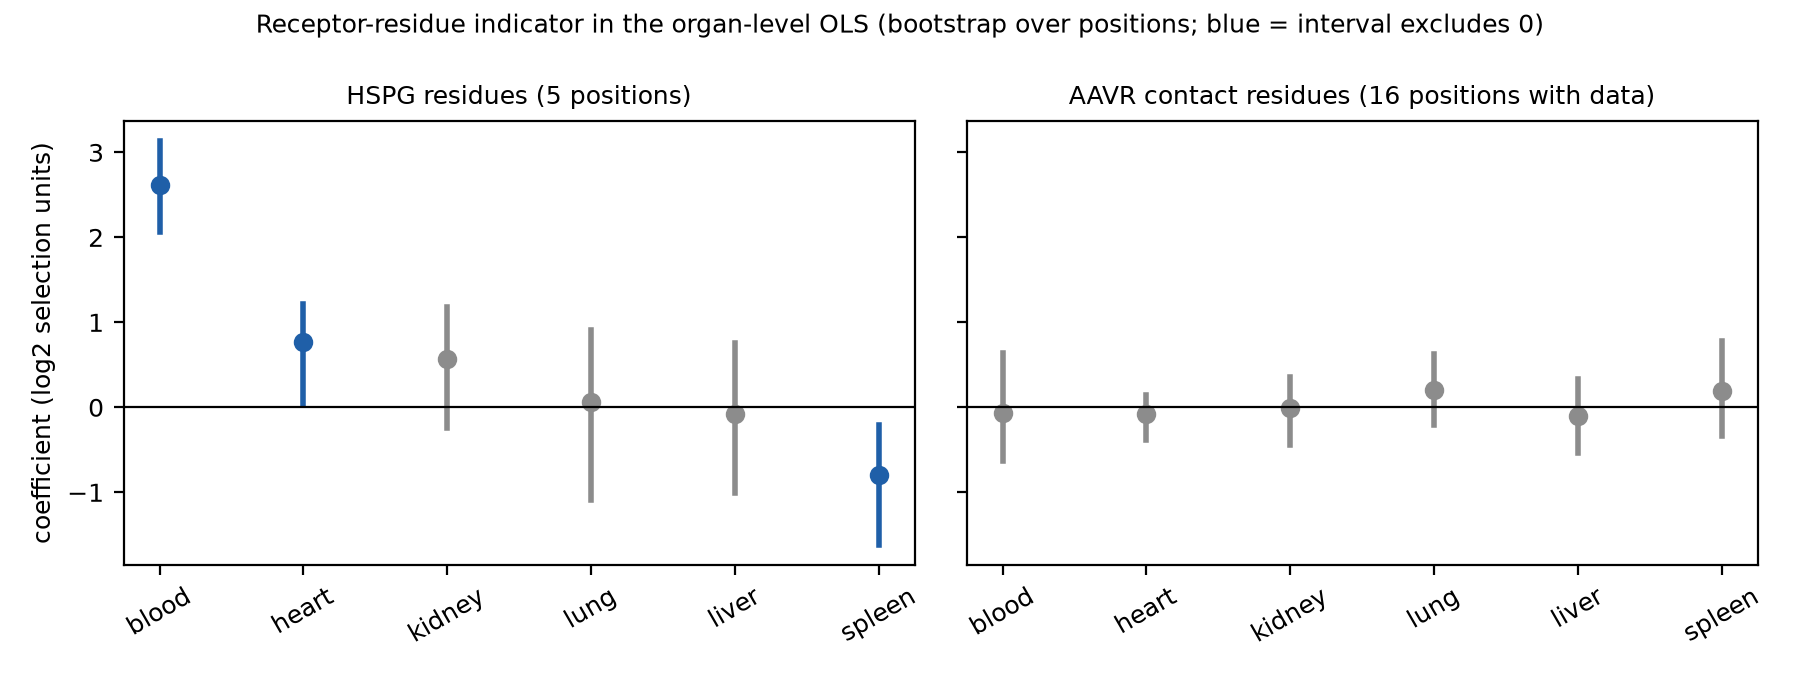
\includegraphics[width=0.95\textwidth]{report_figures/receptor_indicator_coefficients.png}
\caption{The coefficients in Table~\ref{tab:rols}. Blue: interval excludes zero.}
\label{fig:rcoef}
\end{figure}

\textbf{AAVR residues.} No tissue shows an AAVR-residue effect beyond the VR effects
(Table~\ref{tab:rols}: all six intervals include zero, with point estimates between $-$0.11 and
+0.20). At the position level, mean absolute selection is 1.04 vs.\ 0.98 for region-matched
residues ($p=0.51$); heart ($-$0.90 vs.\ $-$0.70) and liver ($-$1.65 vs.\ $-$1.32) are lower at
$p=0.057$ each, and no tissue reaches 0.05. Four of the six scanned VR-I positions are in the
AAVR set, so the VR-I and AAVR terms cannot be separated well: the stable VR-I coefficients in
kidney, liver and spleen are no longer stable when the receptor terms are added. Three listed
residues have no mutants, and 9 of the 16 positions with data have three or fewer, so the power
to detect a per-residue effect is low.

\textbf{VR-VIII.} Table~\ref{tab:rvr8} compares the VR-VIII coefficients from the position-level
bootstrap with and without the receptor terms. Blood, heart and kidney decrease when the HSPG
term is added (blood 1.26 to 1.04, heart 0.29 to 0.23, kidney 0.62 to 0.56), and the heart
interval then reaches zero. Lung, liver and spleen are essentially unchanged (lung $-$0.76 to
$-$0.78, liver $-$0.51 to $-$0.49, spleen $-$0.70 to $-$0.65) and remain stable. So the negative
lung, liver and spleen component of VR-VIII is not carried by R585 and R588.
Figure~\ref{fig:vr8} shows the per-position profile (substitutions only). Blood is highest at 585
and 588 (2.7), and several nearby positions are also positive (583: 1.5, 584: 0.8, 586: 1.2, 590:
1.0); the remaining positions range from $-$1.9 to 0.3. Heart and kidney are positive at 585 and
588 (0.5 to 0.6) and at 583 (0.1 heart, 0.5 kidney) and near or below zero elsewhere. Lung, liver
and spleen are negative at nearly every position.

\begin{table}[H]
\centering
\caption{VR-VIII coefficient in the organ-level OLS with the bootstrap taken over positions,
without and with the HSPG and AAVR indicators (bootstrap mean and 95\% interval). Bold: interval
excludes zero.}
\label{tab:rvr8}
\small
\begin{tabular}{lll}
\toprule
Tissue & Without receptor terms & With receptor terms \\
\midrule
Blood & \textbf{1.26 [0.85, 1.67]} & \textbf{1.04 [0.71, 1.40]} \\
Heart & \textbf{0.29 [0.06, 0.51]} & 0.23 [$-$0.00, 0.45] \\
Kidney & \textbf{0.62 [0.31, 0.93]} & \textbf{0.56 [0.26, 0.88]} \\
Lung & \textbf{$-$0.76 [$-$1.16, $-$0.39]} & \textbf{$-$0.78 [$-$1.18, $-$0.38]} \\
Liver & \textbf{$-$0.51 [$-$0.85, $-$0.21]} & \textbf{$-$0.49 [$-$0.83, $-$0.16]} \\
Spleen & \textbf{$-$0.70 [$-$1.01, $-$0.38]} & \textbf{$-$0.65 [$-$0.96, $-$0.32]} \\
\bottomrule
\end{tabular}
\end{table}

\begin{figure}[H]
\centering
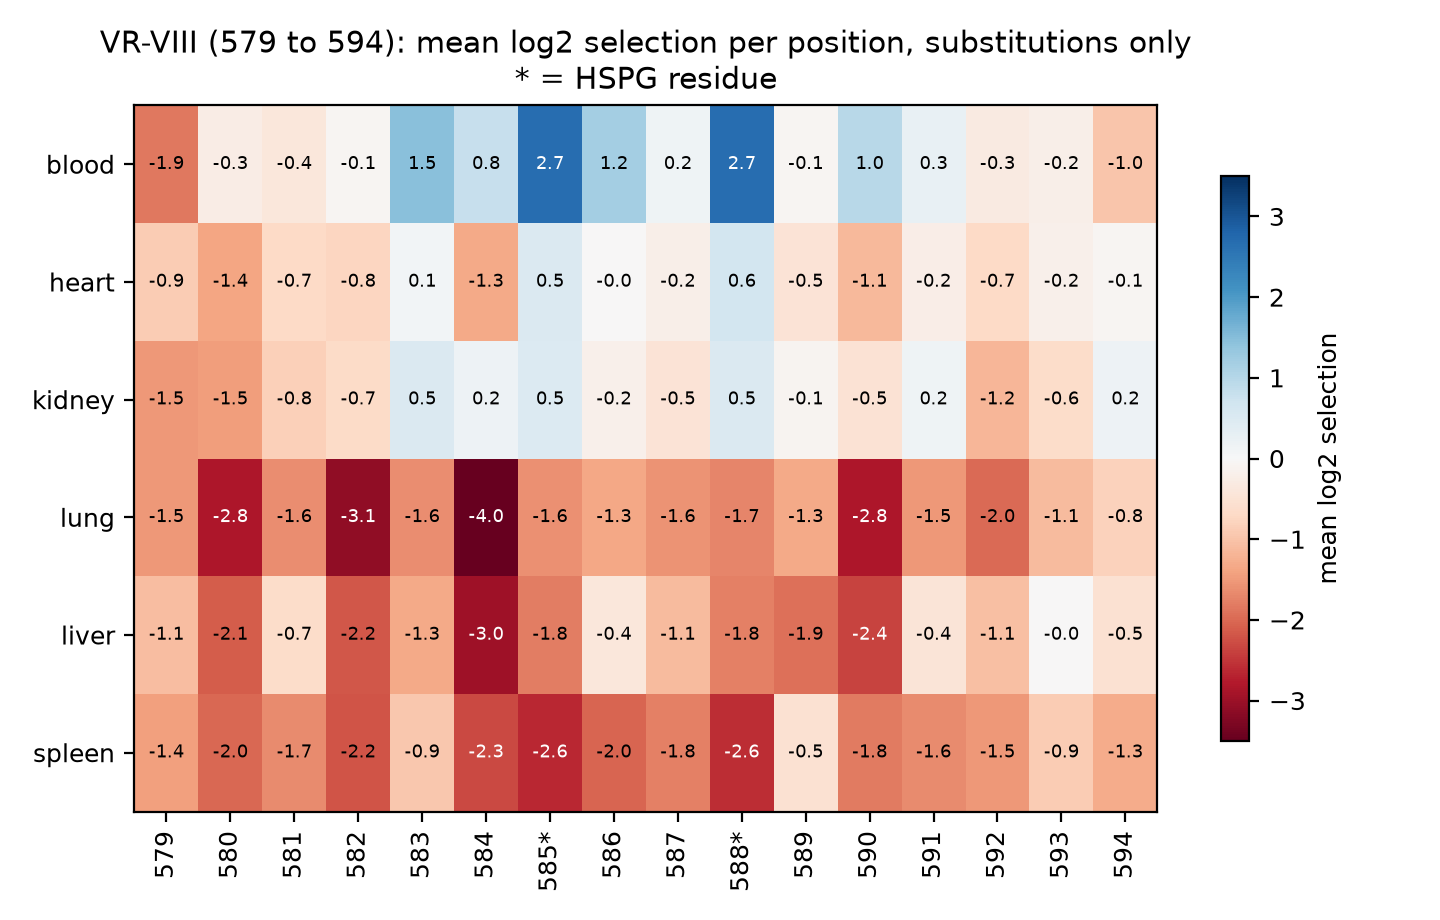
\includegraphics[width=0.85\textwidth]{report_figures/vr8_position_profile.png}
\caption{Mean log2 selection per tissue at each VR-VIII position, substitution mutants only.
Asterisks mark the HSPG residues R585 and R588.}
\label{fig:vr8}
\end{figure}

\textbf{Summary of this section.}
\begin{itemize}
\item The HSPG residues differ from their region-mates in blood (higher), heart (higher) and
  spleen (lower). The direction is what would be expected if less HSPG binding leaves more
  vector in circulation and less taken up by tissue. That expectation comes from the literature;
  the data here do not test it.
\item In liver the HSPG residues are not distinguishable from region-mates.
\item The AAVR residues show no tissue effect beyond the region. AAVR has been reported to be
  required for AAV infection in cell lines and in mice \citep{pillay2016}, which would not predict
  a tissue-specific pattern, but the number of mutants here is too small to tell an absent effect
  from an undetected one.
\item An AAV2 variant with residues 585 to 590 replaced by AAV8 residues (AAV2i8) was reported to
  have about 40-fold lower liver targeting and to target heart and skeletal muscle
  \citep{asokan2010}. The heart direction at R585 and R588 here is the same. The liver result
  here is not specific to those residues.
\item These results are associations at 5 HSPG positions. No test of mechanism was done. Other
  reported AAV2 co-receptors (integrin, FGFR1, laminin receptor, c-Met) were not analyzed
  because we did not have verified residue-level footprints for them.
\end{itemize}

\subsection{PCovC and PCA embeddings}

The embeddings and cross-validated scores below concern the six-tissue selection profiles, not
the mutation features. Figure~\ref{fig:embed} shows the PCA embedding and PCovC embeddings at
three mixing values, colored by the paper's clusters. Table~\ref{tab:ncv} gives $k$-nearest
neighbor accuracy and silhouette score for two label sets: the paper's clusters (which were
themselves derived from PCA and K-means on the same data) and an independent label, the tissue
with the largest absolute deviation for each mutant. The embedding was refit inside each training
fold. Values are the mean over 100 folds (5 folds, 20 repeats) with the 2.5th to 97.5th
percentile of the fold values in brackets; the brackets show the spread of fold scores, not a
confidence interval on the mean.

Against the paper's clusters, PCovC at mixing 0.5 gives kNN accuracy 0.957 vs.\ 0.952 for PCA,
and silhouette 0.059 vs.\ 0.035; the fold ranges overlap. Silhouette rises as mixing decreases
(0.175 at mixing 0). Against the independent label, PCovC at mixing 0.5 and PCA are similar
(kNN 0.584 vs.\ 0.583; silhouette $-$0.180 vs.\ $-$0.191). At mixing 0 the independent-label kNN
accuracy is 0.683 [0.601, 0.738] vs.\ 0.583 for PCA. In a 500-draw label-permutation test at
mixing 0.5, both label sets score above every permuted draw ($p=0.002$). Changing the classifier
inside PCovC (logistic regression, LDA, linear SVC, ridge) changed kNN accuracy by at most 0.006
for the paper's clusters and 0.019 for the independent label
(\texttt{classifier\_sensitivity.csv}).

\begin{figure}[H]
\centering
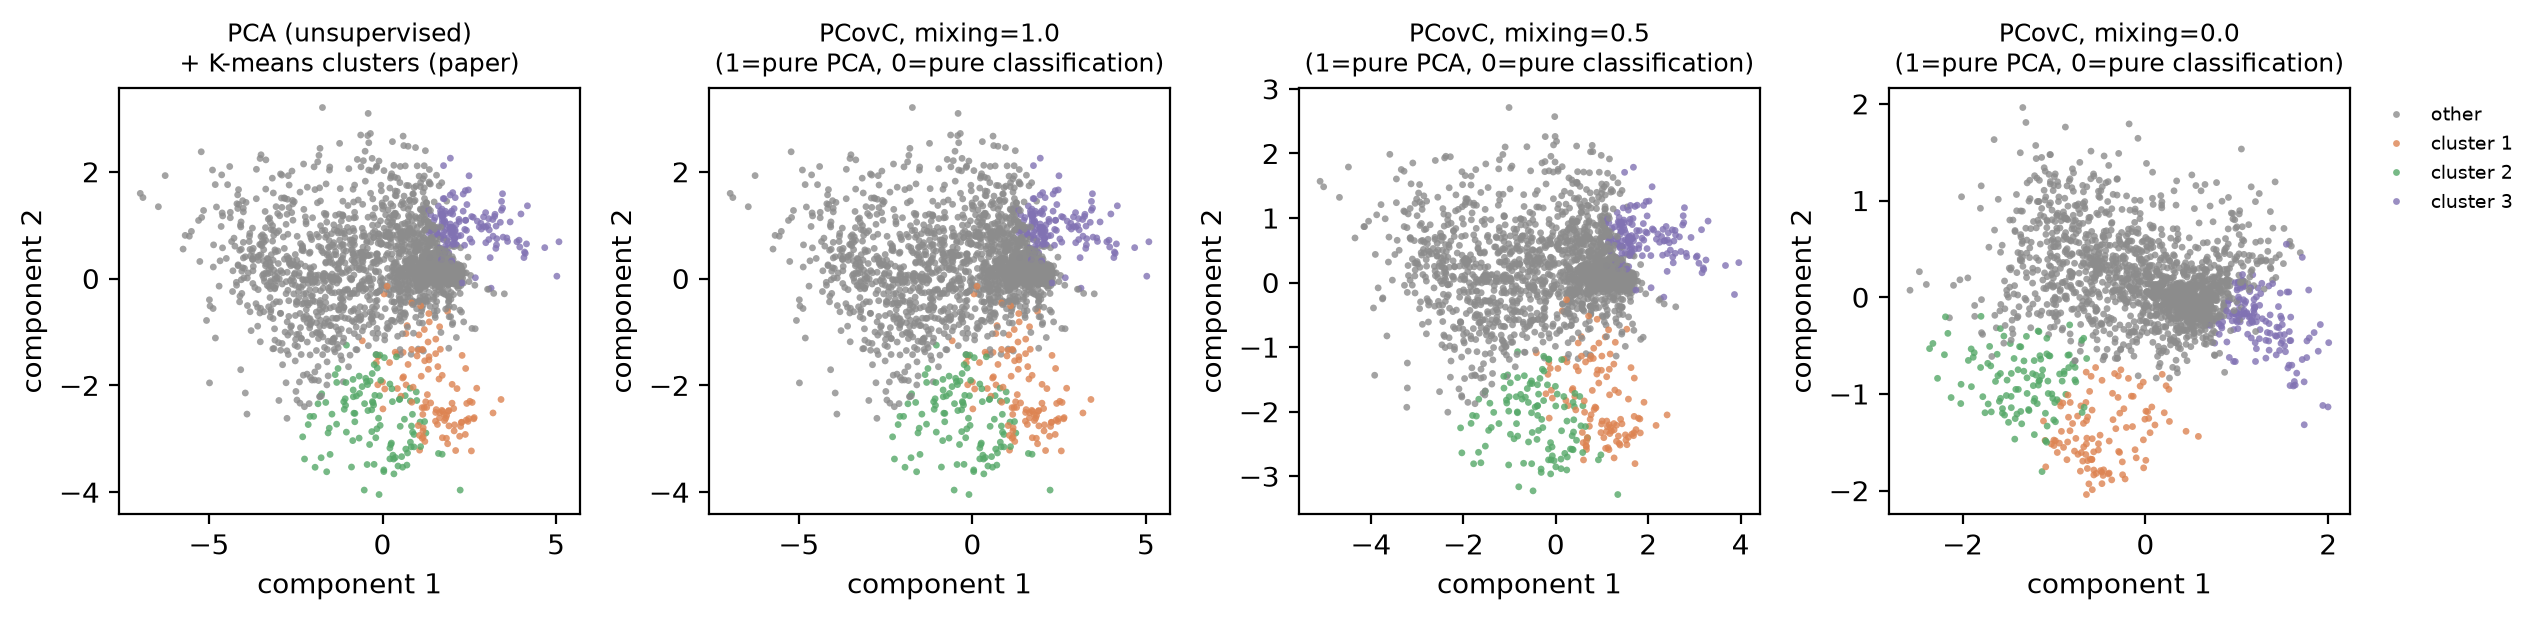
\includegraphics[width=\textwidth]{report_figures/pcovc_vs_pca_comparison.png}
\caption{PCA and PCovC (mixing 1.0, 0.5, 0.0) embeddings of the six-tissue log2 selection
profiles, colored by the paper's clusters.}
\label{fig:embed}
\end{figure}

\begin{table}[H]
\centering
\caption{Nested cross-validated kNN accuracy and silhouette score by method and label set.}
\label{tab:ncv}
\small
\begin{tabular}{llcc}
\toprule
Labels & Method & kNN accuracy & Silhouette \\
\midrule
Paper clusters & PCA & 0.952 [0.935, 0.969] & 0.035 [$-$0.010, 0.078] \\
 & PCovC, mixing 0.00 & 0.960 [0.941, 0.975] & 0.175 [0.113, 0.227] \\
 & PCovC, mixing 0.10 & 0.964 [0.950, 0.978] & 0.129 [0.071, 0.177] \\
 & PCovC, mixing 0.25 & 0.961 [0.945, 0.976] & 0.089 [0.034, 0.137] \\
 & PCovC, mixing 0.50 & 0.957 [0.943, 0.973] & 0.059 [0.009, 0.107] \\
 & PCovC, mixing 0.75 & 0.954 [0.936, 0.970] & 0.044 [$-$0.003, 0.088] \\
 & PCovC, mixing 0.90 & 0.952 [0.936, 0.968] & 0.038 [$-$0.007, 0.081] \\
 & PCovC, mixing 1.00 & 0.952 [0.935, 0.969] & 0.035 [$-$0.010, 0.078] \\
\midrule
Tissue of max deviation & PCA & 0.583 [0.547, 0.625] & $-$0.191 [$-$0.285, $-$0.092] \\
 & PCovC, mixing 0.00 & 0.683 [0.601, 0.738] & $-$0.035 [$-$0.082, 0.011] \\
 & PCovC, mixing 0.10 & 0.639 [0.593, 0.678] & $-$0.086 [$-$0.146, $-$0.035] \\
 & PCovC, mixing 0.25 & 0.568 [0.527, 0.611] & $-$0.153 [$-$0.234, $-$0.074] \\
 & PCovC, mixing 0.50 & 0.584 [0.549, 0.623] & $-$0.180 [$-$0.273, $-$0.088] \\
 & PCovC, mixing 0.75 & 0.584 [0.540, 0.628] & $-$0.188 [$-$0.282, $-$0.093] \\
 & PCovC, mixing 0.90 & 0.583 [0.552, 0.623] & $-$0.190 [$-$0.284, $-$0.092] \\
 & PCovC, mixing 1.00 & 0.583 [0.547, 0.625] & $-$0.191 [$-$0.285, $-$0.092] \\
\bottomrule
\end{tabular}
\end{table}

\section{Limitations and open items}
\label{sec:limits}

\begin{itemize}
\item Bootstrap resamples in the OLS, $p_{xz}$ and Table~\ref{tab:vrorgan} results are drawn over
  mutants. Mutants at the same position share structural context and are not independent, so
  those intervals are probably too narrow. Resampling by position was done only for the VR
  coefficients and the receptor model (Section~\ref{sec:receptor}); there, 30 of 48 VR
  coefficients are stable rather than 35. The property-delta and $p_{xz}$ results have not been rerun
  by position.
\item The position-level tests treat positions as independent. VR positions are contiguous in
  sequence.
\item The 138 OLS coefficients and 100 $p_{xz}$ weights are not corrected for multiple
  comparisons. A stable coefficient means only that its bootstrap interval excludes zero.
\item The 2-fold axis (n=4), VR-II (n=1), VR-I and VR-IX (n=6 each) and deletions (n=37) are
  small groups.
\item The $R^2$ comparison is in-sample and between non-nested feature sets.
\item The position-level and model-level results for VR-VII have not been reconciled.
\item The substitution/insertion sign difference in the centrality relationship has no
  explanation yet.
\item VR boundaries are taken from the authors' code and were not re-derived from the structure.
  VR-III is excluded.
\item The receptor residue sets rest on 5 (HSPG) and 16 (AAVR, with data) positions. The AAVR
  contact list was read from the article page of Meyer et al.\ (Table~2). The HSPG results of Opie
  et al.\ and Kern et al., and the Asokan et al.\ and Pillay et al.\ results cited in
  Section~\ref{sec:receptor}, were taken from abstracts or search summaries, not from the full
  texts.
\item Axis membership, RSA and centrality come from a single structure (1LP3) and one contact
  table. No 3D rendering of any result has been made.
\end{itemize}

\section{Files}

Scripts and outputs are in \texttt{pcovc\_analysis/} and \texttt{pcovc\_analysis/deep\_dive/}
under the project directory. Figures used here are copied to \texttt{report\_figures/}.
Tables in this document were generated from the CSVs in \texttt{deep\_dive/} by a script, not
typed by hand.

\begin{thebibliography}{99}

\bibitem[Ogden et al.(2019)]{ogden2019} Ogden PJ, Kelsic ED, Sinai S, Church GM. Comprehensive AAV
capsid fitness landscape reveals a viral gene and enables machine-guided design. \textit{Science}
366(6469):1139--1143 (2019).

\bibitem[Jorgensen et al.(2026)]{jorgensen2026} Jorgensen C, Lin AY, Vasavada R, Cersonsky RK.
Interpretable Visualizations of Data Spaces for Classification Problems. \textit{Mach. Learn.:
Sci. Technol.} 7(2):025008 (2026).

\bibitem[Goscinski et al.(2023)]{goscinski2023} Goscinski A, Principe VP, Fraux G, et al.
scikit-matter: a suite of generalisable machine learning methods born out of chemistry and
materials science. \textit{Open Res. Europe} (2023).

\bibitem[Xie et al.(2002)]{xie2002} Xie Q, Bu W, Bhatia S, Hare J, Somasundaram T, Azzi A,
Chapman MS. The atomic structure of adeno-associated virus (AAV-2), a vector for human gene
therapy. \textit{Proc. Natl. Acad. Sci. USA} 99(16):10405--10410 (2002). PDB 1LP3.

\bibitem[Bleker et al.(2005)]{bleker2005} Bleker S, Sonntag F, Kleinschmidt JA. Mutational
Analysis of Narrow Pores at the Fivefold Symmetry Axes of Adeno-Associated Virus Type 2 Capsids
Reveals a Dual Role in Genome Packaging and Activation of Phospholipase A2 Activity. \textit{J.
Virol.} 79(4):2528--2540 (2005).

\bibitem[Mietzsch et al.(2019)]{mietzsch2019} Mietzsch M, Penzes JJ, Agbandje-McKenna M.
Twenty-Five Years of Structural Parvovirology. \textit{Viruses} 11(4):362 (2019).

\bibitem[Opie et al.(2003)]{opie2003} Opie SR, Warrington KH Jr, Agbandje-McKenna M, Zolotukhin S,
Muzyczka N. Identification of amino acid residues in the capsid proteins of adeno-associated virus
type 2 that contribute to heparan sulfate proteoglycan binding. \textit{J. Virol.}
77(12):6995--7006 (2003).

\bibitem[Kern et al.(2003)]{kern2003} Kern A, Schmidt K, Leder C, Muller OJ, Wobus CE, Bettinger K,
Von der Lieth CW, King JA, Kleinschmidt JA. Identification of a heparin-binding motif on
adeno-associated virus type 2 capsids. \textit{J. Virol.} 77(20):11072--11081 (2003).

\bibitem[Meyer et al.(2019)]{meyer2019} Meyer NL, Hu G, Davulcu O, Xie Q, Noble AJ, Yoshioka C,
Gingerich DS, Trzynka A, David L, Stagg SM, Chapman MS. Structure of the gene therapy vector,
adeno-associated virus with its cell receptor, AAVR. \textit{eLife} 8:e44707 (2019).

\bibitem[Asokan et al.(2010)]{asokan2010} Asokan A, Conway JC, Phillips JL, et al. Reengineering a
receptor footprint of adeno-associated virus enables selective and systemic gene transfer to
muscle. \textit{Nat. Biotechnol.} 28:79--82 (2010).

\bibitem[Pillay et al.(2016)]{pillay2016} Pillay S, Meyer NL, Puschnik AS, et al. An essential
receptor for adeno-associated virus infection. \textit{Nature} 530:108--112 (2016).

\end{thebibliography}

\end{document}
